\documentclass[preprint]{sigplanconf}
\usepackage{version}
\usepackage[pdftex]{graphicx}
\usepackage{amsmath}
\usepackage{amsfonts,amssymb}
\usepackage{style/utils}
\usepackage{style/code}
\usepackage{alltt}
\usepackage{stmaryrd}
\usepackage{url}
\usepackage{graphicx}

\newcommand{\comm}[1]{\textrm{--- {#1}}}
\newcommand{\tup}[1]{\overline{#1}}

% Program font stuff
\newcommand{\ccode}[1]{\texttt{#1}}
\newcommand{\hskwd}[1]{\texttt{#1}}
\newcommand{\hslam}[1]{\ensuremath{\lambda}}
\newcommand{\capp}{\texttt{\$\!:}}
\newcommand{\cappP}{\mathbin{{\$}{:}^\uparrow}}

% Notation for type-indexed parallel arrays
\newcommand{\pacls}{\texttt{PA}}        % Parallel array class
\newcommand{\pacon}{\texttt{PArray}}    % Parallel array data type family
\newcommand{\pa}[1]{\pacon\;#1}         % PArr in *vectorised* code
\newcommand{\paB}[1]{(\pa{#1})}         % Bracketed PArr in *vectorised* code

\newcommand{\patype}[1]{\mathsf{patype}\langle#1\rangle}  % Not sure about this

\newcommand{\inform}[1]{\ensuremath{\langle\textrm{#1}\rangle}}
\newcommand{\var}[1]{\ensuremath{\mathit{#1}}}
\newcommand{\sub}[1]{\ensuremath{_{\mathnormal{#1}}}}
\newcommand{\LV}[1]{#1\ensuremath{_{\mathrm{L}}}}
\newcommand{\VV}[1]{#1\ensuremath{_{\mathrm{V}}}}
\newcommand{\SE}[1]{#1\ensuremath{_{\mathrm{S}}}}
\newcommand{\Arr}[1]{#1$_{\code{\pacon}}$}

\newcommand{\meta}[1]{\ensuremath{\llbracket\text{#1}\rrbracket}}
\newcommand{\TT}[1]{\ensuremath{\mathcal{V}_t\llbracket #1 \rrbracket}}
\newcommand{\TTL}[1]{\ensuremath{\mathcal{L}_t\llbracket #1 \rrbracket}}
\newcommand{\VT}[1]{\ensuremath{\mathcal{V}\left\llbracket #1 \right\rrbracket}}
\newcommand{\LT}[2]{\ensuremath{\mathcal{L}\left\llbracket #2 \right\rrbracket\,#1}}
\newcommand{\LTprime}[2]{\ensuremath{\mathcal{L}'\left\llbracket #2 \right\rrbracket\,#1}}

\newcommand{\AV}[2]{\ensuremath{\mathcal{A}\left\llbracket #1 \right\rrbracket\,#2}}
\newcommand{\AT}[1]{\ensuremath{\mathcal{A}_T\left\llbracket #1 \right\rrbracket}}
\newcommand{\AVP}{\ensuremath{\mathbf{p}}}
\newcommand{\AVC}{\ensuremath{\mathbf{c}}}
\newcommand{\AVS}{\ensuremath{\mathbf{s}}}
\newcommand{\AVE}{\ensuremath{\mathbf{e}}}
\newcommand{\orp}{\ensuremath{\rhd}}

\newcommand{\Encaps}[1]{\ensuremath{\mathcal{E}\left\llbracket #1 \right\rrbracket}}
\newcommand{\VE}[1]{\ensuremath{\mathcal{VE}\left\llbracket #1 \right\rrbracket}}
\renewcommand{\textfraction}{0.2}
\renewcommand{\topfraction}{0.9}
\renewcommand{\dbltopfraction}{0.9}
\renewcommand{\floatpagefraction}{0.9}
\renewcommand{\dblfloatpagefraction}{0.9}
\newcommand{\fvs}[1]{\ensuremath{\mathit{fvs}(#1)}}

% -----------------------------------------------------------------------------
\begin{document}
%\preprintfooter{\textbf{--- DRAFT --- DRAFT --- DRAFT --- DRAFT ---}}

\title  {Vectorisation Avoidance}

\authorinfo
{       Gabriele Keller$^\dagger$
   \and Manuel Chakravarty$^\dagger$ 
   \and Roman Leshchinskiy
   \\[4pt]
        Ben Lippmeier$^\dagger$
   \and Simon Peyton Jones$^\ddagger$
}
{ \vspace{5pt}
  \shortstack{
    $^\dagger$School of Computer Science and Engineering \\
    University of New South Wales, Australia \\[2pt]
    \textsf{\{keller,chak,rl,benl\}@cse.unsw.edu.au}
  }
  \hspace{5em}
  \shortstack{
    $^\ddagger$Microsoft Research Ltd \\
    Cambridge, England \\[2pt]
    \textsf{\{simonpj\}@microsoft.com}
  }
}

\maketitle
\makeatactive


% -----------------------------------------------------------------------------
\begin{abstract}
Flattening nested parallelism is a vectorising code transform that converts irregular nested parallelism into flat data parallelism. Although the result has good asymptotic performance, flattening thoroughly restructures the code. Many intermediate data structures and traversals are introduced, which may or may not be eliminated by subsequent optimisation. We present a novel program analysis to identify parts of the program where flattening would only introduce overhead, without appropriate gain. We present empirical evidence that avoiding vectorisation in these cases leads to more efficient programs than if we had applied vectorisation and then relied on array fusion to eliminate intermediates from the resulting code.
\end{abstract}

\category
	{D.3.3}
	{Programming Languages}
	{Language Constructs and Features---Concurrent programming structures; Polymorphism; Abstract data types}

\terms
	Languages, Performance

\keywords
	Nested data parallelism, Haskell, Program transformation


% -----------------------------------------------------------------------------
\section{Introduction}

Data Parallel Haskell (DPH) is an extension to the Glasgow Haskell Compiler (GHC) that implements \emph{nested data parallelism}. DPH is based on a vectorising program transformation called \emph{flattening}~\cite{blelloch-sabot:compiling-collection, keller-chak:tflat, chak-keller:more-types, leshchinskiy-etal:ho-flattening, Jones08harnessingthe}, which converts irregular and nested data parallelism into regular traversals over multiple flat arrays. Flattening simplifies load balancing and enables SIMD parallelism together with cache-friendly, linear traversals of unboxed arrays. 

Unfortunately, without subsequent aggressive optimisation, flattened code is grossly inefficient on current computer architectures. A key aspect of flattening is to convert \emph{scalar operations} into aggregate \emph{array operations} --- such as turning floating-point addition into the pairwise addition of two arrays of floats. However, intermediate scalar values in the source code are also converted to arrays, so values that were once stored in scalar registers are now shuffled to and from memory between each array operation.

The observation that flattening increases memory traffic is not new~\cite{so-etal:dp-many-core, chak:functional-array-fusion, chak-etal:partial-vectorisation, chak-etal:status-report}, and DPH uses array fusion~\cite{coutts:rewriting-strings, coutts:stream-fusion} to try and combine successive array operations back into a single traversal. While this works for small kernels, relying on fusion alone turned out to have four serious drawbacks:
%
\begin{enumerate}
\item Array fusion can be fragile, as it depends on many enabling code transformations.

\item Specifically, fusion depends critically on inlining --- which must be conservative in the presence of sharing to avoid work duplication, and cannot handle recursive definitions.

\item Aggressive inlining leads to large intermediate programs, and hence long compile times.

\item Even if fusion goes well, GHC's current back-end code generators cannot properly optimise fused code, which leads to excessive register use in the resulting machine code.
\end{enumerate}

On closer inspection, we have identified many common situations in which vectorisation provides no benefit, though the overheads introduced are very much apparent. Thus motivated, we present a program analysis that allows us to completely avoid vectorising parts of the program that do not require it. To our knowledge, this is the first attempt to guide flattening-based vectorisation so that vectorisation is avoided where it is not needed, instead of relying on a subsequent fusion stage to clean up afterwards. 

In summary, we make the following contributions:
%
\begin{itemize}
\item We characterise those parts of DPH programs where vectorisation introduces overheads, without appropriate gain (Section~\ref{Section:too-much} \&~\ref{Section:Vectorisation}).

\item We introduce a program analysis to identify subexpressions that need not be vectorised and modify the flattening transform to lift entire expressions to vector-space, which avoids converting its intermediates to array values. (Section~\ref{Section:NewTrafo}).

\item We present empirical evidence that supports our claim that vectorisation avoidance is an improvement over plain array fusion, at least for our benchmarks (Section~\ref{Section:Performance})
\end{itemize}
%

In our previous work~\cite{chak-etal:partial-vectorisation} we introduced \emph{partial vectorisation}, which allows vectorised and unvectorised code to be combined in the same program. With partial vectorisation, the unvectorised portion fundamentally \emph{cannot} be vectorised, such as when it performs an IO action. In contrast, this paper presents \emph{vectorisation avoidance}, where the unvectorised portion is code that \emph{could} be vectorised, but we choose not to for performance reasons. We discuss further related work in Section~\ref{sec:related}.

\eject
\section{Too Much Vectorisation}
\label{Section:too-much}

Vectorisation for higher-order programs is a complex transformation, but we only need the basics to appreciate the problem addressed in this paper. In this section, we walk though a simple example that highlights the problem with intermediate values, and sketch our solution.

% -----------------------------------------------------------------------------
\subsection{Parallel force calculation}

We use a parallel gravitation simulation as a running example. The simulation consists of many massive points (bodies), each with a mass, a location in two dimensions, and a velocity vector: 
%
\begin{small}
\begin{alltt}
  type Mass      = Float
  type Vector    = (Float, Float)
  type Location  = Vector
  type Velocity  = Vector
  type Accel     = Vector
  data MassPoint = MP Mass Location Velocity
\end{alltt}
\end{small}
%
At each time step we compute the acceleration due to gravitational force between each body, and use the sum of accelerations to update each body's velocity. The following @accel@ function computes the acceleration between two bodies. The @eps@ (epsilon) parameter is a smoothing factor that prevents the acceleration from approaching infinity when the distance between the two bodies approaches zero.
%
\begin{small}
\begin{alltt}
  accel :: Float -> MassPoint -> MassPoint -> Accel                            
  accel eps (MP _ (x1, y1) _) (MP m (x2, y2) _)
   = let dx   = x1 - x2 
         dy   = y1 - y2 
         rsqr = dx * dx + dy * dy + eps * eps
         r    = sqrt rsqr 
         aabs = m  / rsqr
     in  (aabs * dx / r , aabs * dy / r)  
\end{alltt}
\end{small}
%
In DPH we express nested data parallelism using bulk operations on \emph{parallel arrays}. The type of parallel arrays is written @[:e:]@, for some element type @e@. Parallel array operators behave like Haskell's standard list operators (but on arrays), and are identified by a suffix @P@ --- for example, @mapP@, @unzipP@, @sumP@, and so on.  We also use \emph{parallel array comprehensions}, which behave similarly to list comprehensions~\cite{Jones08harnessingthe}.

Using parallel array comprehensions, we implement a na\"ive $O(n^2)$ algorithm that takes a parallel array of bodies, and computes the gravitational acceleration acting on each one:
%
\begin{small}
\begin{alltt}
  allAccels :: Float -> [:MassPoint:] -> [:Accel:]
  allAccels eps mps 
   = [: (sumP xs, sumP ys) 
      | mp1 <- mps
      , let (xs, ys) = unzipP [: accel eps mp1 mp2 
                     | mp2 <- mps :]    
      :]
\end{alltt}
\end{small}
%
The crucial difference between Haskell lists and parallel arrays is that the latter have a parallel evaluation semantics. Demanding any element in a parallel array results in them all being computed, and on a parallel machine we expect this computation to run in parallel.

The degree of parallelism in @allAccels@ is $n^2$, as we use nested parallelism by way of nested array comprehensions to compute all pairwise accelerations in parallel. We also sum the individual accelerations on each body using $2*n$ parallel sums in parallel. In the full simulation we would then use the resulting accelerations to compute new velocities and positions for each body. 

Although this is a na\"ive algorithm, it presents the same challenges with respect to vectorisation of intermediates as the more sophisticated \mbox{Barnes-Hut} algorithm. We stick to the simpler version to avoid complications with the irregular tree structures that \mbox{Barnes-Hut} uses, which are orthogonal to the ideas discussed in this paper.


% -----------------------------------------------------------------------------
\subsection{Lifting functions into vector space}
\label{Subsection:liftedFunctions}

Vectorising @accel@ from the previous section and simplifying yields \texttt{accel\sub{L}} shown below. The subscript $L$ is short for ``lifted'', and we describe vectorisation as \emph{lifting a function to vector space}. 
%
\begin{small}
\begin{alltt}
 accel\sub{L} :: PArray Float 
         -> PArray MassPoint -> PData MassPoint 
         -> PArray Accel
 accel\sub{L} epss (MP\sub{L} _ (xs1,ys1) _) (MP\sub{L} ms (xs2,ys2) _)
  = let dxs   = xs1 -\sub{L} xs2 
        dys   = ys1 -\sub{L} ys2 
        rsqrs = dxs *\sub{L} dxs +\sub{L} dys *\sub{L} dys +\sub{L} epss *\sub{L} epss
        rs    = sqrt\sub{L} rsqrs 
        aabss = ms  /\sub{L} rsqrs 
    in  (aabss *\sub{L} dxs /\sub{L} rs , aabss *\sub{L} dys /\sub{L} rs)  
\end{alltt}
\end{small}
%
In the type of \texttt{accel\sub{L}}, the @PArray@ constructor is our internal version of @[::]@ which only appears in vectorised code. A value of @(PArray a)@ contains elements of type @a@, which are stored in a type-dependent manner. For example, we store an array of pairs of integers as two arrays of unboxed integers. This ``unzipped'' representation avoids the intermediate pointers that would otherwise be required in a completely boxed representation. Similarly, we store an array of @MassPoint@ as five separate arrays: an array of masses, two arrays for the $x$ and $y$ components of their locations, and two arrays for the $x$ and $y$ components of their velocities. We can see this in the above code, where we add as @s@ suffix to variable names to highlight that they are now array-valued.
%
% We can see this in the code above, where the lifted @MP@ constructor \texttt{MP\sub{L}} has the following type:
% \begin{small}
% \begin{alltt}
%    MP\sub{L} :: PData Mass 
%         -> (PData Float, PData Float) 
%         -> (PData Float, PData Float)
%         -> PData MassPoint
% \end{alltt}
% \end{small}
%

Lifting of @accel@ itself is straightforward, as it is one big arithmetic expression without any interesting control flow. The lifted versions of primitive functions are just like their originals, except they operate on arrays of values. For example:
%
\begin{small}
\begin{alltt}
  (*\sub{L}) :: PArray Float -> PArray Float -> PArray Float
\end{alltt}
\end{small}

Pairwise multiplication operates as \texttt{(*\sub{L}) = zipWithP (*)} and is provided by the back-end DPH libraries, along with other lifted primitives.

Returning to the definition of \texttt{accel\sub{L}} we see the problem with intermediate values. Whereas the variables @rsqr@, @r@, @dx@, @dy@ and so on were scalar values in the source code, in the lifted version they have become array values. Without array fusion, each of these intermediate arrays will be reified in memory, whereas with the unvectorised program they would exist only transiently in scalar registers. 

As the original @accel@ function does not use nested parallelism, branching, or anything else that justifies an elaborate transformation, we might have hoped for simpler code. Actually, we would like the vectoriser to produce the following instead:
% Strictly speaking, the lifted code generated by higher-order vectorisation is more involved. However, as the example makes no use of higher-order features, after some simplifcations, the code is as above. It highlights the core of the problem that we strive to solve in the present paper: several intermediate parallel arrays are created (by the lifted arithmetic operations) and, for example in the case of @dxs@ and @dys@, traversed multiple times. Inlining and fusion could eliminate some of that, but not all. Since we can see that there is no nested parallelism or anything else that justifies an elaborate transformation, we might have hoped for simpler code. %
%
\begin{small}
\begin{alltt}
  accel\sub{L} epss (MP\sub{L} _ (xs1,ys1) _) (MP\sub{L} ms (xs2,ys2) _)
   = let f eps x1 y1 x2 y2 m
           = let dx   = ...; dy = ...; 
                 rsqr = ...; r  = ...; aabs = ...
                 \(\ldots\langle\textrm{as in original definition of \texttt{accel}}\rangle\ldots\)
             in  (aabs * dx / r , aabs * dy / r)
     in  zipWithPar6 f epss xs1 ys1 xs2 ys2 ms
\end{alltt}
\end{small}
Here, @zipWithPar6@ is a 6-ary parallel-array variant of @zipWith@. This simpler version of \texttt{accel\sub{L}} performs just one single simultaneous traversal of all six input arrays, without producing any unnecessary array-valued intermediates. 

Importantly, we can create this simpler version of \texttt{accel\sub{L}} only because the original version \emph{does not directly nor indirectly call any parallel functions}. This property ensures that the use of @zipWithPar6@ does not introduce any nested parallelism itself. If the original @accel@ used a data-parallel function, then it would need to be called for each pair of points --- and this is precisely what flattening is supposed to eliminate.

\eject
So the question is this: can we identify \emph{purely-sequential sub-computations} (such as @accel@) that will not benefit from vectorisation?  If so, we can generate simple, efficient @zipWith@-style loops for these computations, instead of applying the general vectorisation transformation and hoping that fusion then eliminates the intermediate arrays it introduces. 


% -----------------------------------------------------------------------------
\subsection{Maximal sequential subexpressions}
\label{sec:maximal-seq}

The situation in the previous section was the ideal case. With @accel@ we were able to avoid vectorising its entire body because it did not use any data parallel functions. This made @accel@ completely sequential. Usually we are not that lucky, and the function we want to vectorise contains parallel subexpressions as well as sequential ones. In general, to perform vectorisation avoidance we need to identify \emph{maximal sequential subexpressions}, which are sequential subexpressions that encompass as many operations as possible.

To illustrate this idea, consider a variant of @accel@, where the smoothing factor is not passed as an argument, but instead determined by a parallel computation that references @dx@ and @dy@:
%
\begin{small}
\begin{alltt}
  accel' (MP _ (x1, y1) _) (MP m (x2, y2) _)
   = let dx   = x1 - x2 
         dy   = y1 - y2 
         eps  = \(\langle\textrm{a data-parallel computation with dx and dy}\rangle\)
         rsqr = dx * dx + dy * dy + eps * eps
         r    = sqrt rsqr 
         aabs = m / rsqr 
     in  (aabs * dx / r , aabs * dy / r)
\end{alltt}
\end{small}

This time we cannot lift @accel'@ by wrapping the entire body in a parallel zip, as this would yield a nested parallel computation. Instead, we proceed as follows: (1) identify all maximal sequential subexpressions; (2) lambda lift each of them, and (3) use @zipWithPar@$n$ to apply each lambda lifted function element-wise to its lifted (vectorised) free variables. Doing this to the above function yields:

% \begin{small}
% \begin{alltt}
% accel'\sub{L} (MP\sub{L} _ (xs1, ys1) _) (MP\sub{L} ms (xs2, ys2) _)
%  = let dxs   = zipWithPar  (\(\lambda\)x1 x2. x1 - x2)   xs1 xs2 
%        dys   = zipWithPar  (\(\lambda\)y1 y2. y1 - y2)   ys1 ys2
%        epss  = \(\langle\textrm{lifted data-parallel computation}\rangle\) 
%        rsqrs = zipWithPar3 (\(\lambda\)dx dy eps. 
%                  dx * dx + dy * dy + eps * eps) 
%                  dxs dys epss
%        rs    = mapPar      (\(\lambda\)rsqr. sqrt rsqr)  rsqrs 
%        aabss = zipWithPar  (\(\lambda\)m rsqr. m / rsqr) ms rsqrs
%    in  zipWithPar4 (\(\lambda\)aabs dx dy r. 
%          (aabs *  dx / r, aabs * dy / r))  
%          aabss dxs dys rs
% 
% \end{alltt}
% \end{small}

\begin{small}
\begin{alltt}
 accel'\sub{L} (MP\sub{L} _ (xs1, ys1) _) (MP\sub{L} ms (xs2, ys2) _)
   = let dxs   = zipWithPar (\(\lambda\)x1 x2. x1 - x2) xs1 xs2 
         dys   = zipWithPar (\(\lambda\)y1 y2. y1 - y2) ys1 ys2
         epss  = \(\langle\textrm{lifted data-parallel computation with dxs and dys}\rangle\) 
     in  zipWithPar4 (\(\lambda\)m dx dy eps. 
           let rsqr = dx * dx + dy * dy + eps * eps
               r    = sqrt rsqr
               aabs = m / rsqr
           in  (aabs * dx / r, aabs * dy / r))
           ms dxs dys epss
\end{alltt}
\end{small}
%
The resulting lifted function \texttt{accel'\sub{L}} contains three parallel array traversals, whereas \texttt{accel\sub{L}} only had one. Nevertheless, that is still much better than the 13 traversals that would be in the vectorised code without vectorisation avoidance.

We were able to \emph{encapsulate} the bindings for @rsqr@, @r@, and @aabs@ by the final traversal because after the @eps@ binding, there are no more parallel functions. In general, we get the best results when intermediate sequential bindings are floated close to their use sites, as this makes them more likely to be encapsulated along with their consumers.


% -----------------------------------------------------------------------------
\subsection{Conditionals and recursive functions}
\label{sec:conditionals}

The function @accel@ didn't have any control flow constructs. For an example with a conditional, consider a division function that tests for a zero divisor:
%
\begin{small}
\begin{alltt}
  divz :: Float -> Float -> Float
  divz x y = if (y == 0)
              then 0   
              else x `div` y
\end{alltt}
\end{small}
%
To vectorise a conditional we first compute an array of flags indicating which branch to take for each iteration. We use these flags to split the array valued free variables into the elements for each branch, and apply the lifted version of each branch to just those elements associated with it. Finally, we re-combine the results of each branch using the original array of flags. Without vectorisation avoidance, the lifted version of @divz@ is as follows:
%
\begin{small}
\begin{alltt}
  divz\sub{L} :: PArray Float -> PArray Float -> PArray Float
  divz\sub{L} xs ys 
   = let n               = lengthPA ys
         flags           = (ys ==\sub{L} (replicatePA n 0))
         (xs\sub{then}, xs\sub{else}) = splitPA flags xs
         (ys\sub{then}, ys\sub{else}) = splitPA flags ys
     in  combinePA flags (replicatePA (countPA flags) 0)
                         (xs\sub{else} `div`\sub{L} ys\sub{else})
\end{alltt}
\end{small}
%
Using these extra intermediate arrays lets us guarantee that the parallel execution of divz\sub{L} will be load-balanced. To see this, suppose that performing a division on our parallel machine is more expensive than simply returning a constant 0. If we were to evaluate multiple calls to @divz@ in parallel without using our @splitP/combineP@ technique, there is a chance that one processor would need to evaluate more divisions than another, leading to work imbalance. However, in the code above we split the input arrays (@xs@ and @ys@) into the elements corresponding to each branch, and use \emph{all} processors to compute the results for both branches. As all processors are used to evaluate both branches, we can be sure the computation is perfectly balanced.
 
Unfortunately, both @splitP@ and @combineP@ are expensive operations. If we were to execute the unvectorised version of @divz@ then the arguments for @x@ and @y@ would be passed in scalar registers. The flag indicating which branch to take would also be computed in a register. Once again, when we vectorise @divz@ these intermediate values are converted to arrays, which reifies them in memory. On current hardware, the extra memory traffic introduced \emph{for this example} will far exceed the gain from improved load balancing. For this example it is better to avoid vectorising the conditional entirely and instead generate:
%
\begin{small}
\begin{alltt}
  divz\sub{L} xs ys 
   = zipWithPar2 (\(\lambda\)x y.
       if (y == 0) then 0 else x `div` y) 
       xs ys
\end{alltt}
\end{small}
%
The situation becomes even more interesting when recursion is involved, such as in this familiar function:
%
\begin{small}
\begin{alltt}
  fac :: Int -> Int -> Int
  fac acc n 
   = if n == 0 then acc
               else fac (n * acc) (n - 1)
\end{alltt}
\end{small}
%
Lifting this function without vectorisation avoidance will use @splitP@ and @combineP@ to flatten the conditional, and the recursive call will be to the lifted version. The consequence is excessive data movement for each recursion and an inability to use the tail recursion optimisation.

In contrast, using vectorisation avoidance we can confine the recursive call to the sequential portion of the function:
%
\begin{small}
\begin{alltt}
  fac\sub{L} :: PArray Int -> PArray Int -> PArray Int
  fac\sub{L} accs ns
   = let f acc n 
          = if n == 0 then acc
                       else f (n * acc) (n - 1)
     in  zipWithPar2 f xs ys
\end{alltt}
\end{small}
%
This code risks severe load imbalance if the depth of the recursion varies widely among the instances computed on each processor. At the same time, it also avoids the high overheads of the fully vectorised version. Which is the lesser evil?

In our experience so far, using vectorisation avoidance for purely sequential recursive functions has always produced faster code. We intend to provide a pragma to override this default approach in exceptional cases.


% -----------------------------------------------------------------------------
\subsection{Vectorisation avoidance in a nutshell}

In summary, vectorisation avoidance consists of three steps. First, we identify the maximal sequential subexpressions. Second, we lambda lift those subexpressions. Third, we use @zipWithPar@$n$ to apply each lambda-lifted function (in parallel) to each valuation of its free variables. As a result we generate fewer array traversals and fewer intermediate arrays, though we may sacrifice some load balancing by doing so.

As we will see in the next section, the most tricksy step of vectorisation avoidance is the first --- identification of the maximal sequential subexpressions. Once this information has been computed, it is reasonably straightforward to use it in the vectorisation transform itself. We will formalise this process in Section~\ref{Section:NewTrafo}.


\section{Vectorisation Revisited}
\label{Section:Vectorisation}

This section discusses the features of vectorisation that are central to adding vectorisation avoidance. For a complete description of vectorisation, see our previous work~\cite{Jones08harnessingthe}.


% -----------------------------------------------------------------------------
\subsection{Parallel arrays, maps, and the \texttt{Scalar} type class}
\label{sec:flattening-arrays}
\label{Subsection:Scalar}

As mentioned in Section~\ref{Subsection:liftedFunctions}, in vectorised code we store parallel array data in a type-dependent manner, so the representation of @PArray a@ depends on the element type @a@. Haskell, we realise this using type families~\cite{chak-etal:ATs,chak-etal:at-syns} like so:
%
\begin{small}
\begin{alltt}
data family   PArray a
data instance PArray Int        = PInt (Vector Int)
data instance PArray (a, b)     = P2 (PArray a) (PArray b)
data instance PArray (PArray a) = PNested VSegd (PDatas a)
... more instances ...
\end{alltt}
\end{small}

For arrays of primitive values such as @Int@ and @Float@ we use an unboxed representation; specifically, the unboxed arrays from the @vector@ package.\footnote{\url{http://hackage.haskell.org/package/vector}} Using unboxed arrays improves absolute performance over standard boxed arrays, and admits a simple load balancing strategy when consuming them. For structured data we hoist the structure to top-level: representing an array of structured values as a tree with with unboxed arrays of scalars at its leaves. The instance for pairs is shown above. 

The @PArray@ type family also supports flattening of nested arrays, and arrays of sum types~\cite{chak-etal:status-report, Jones08harnessingthe, lippmeier:work-efficient}. A partial definition of nested arrays shown above, but we leave discussion of the @VSegd@ segment descriptor and @PDatas@ data blocks to \cite{lippmeier:work-efficient}. 

For vectorisation avoidance, the important point is that we can only bail out to a sequential function if the elements that function consumes can be extracted from their arrays in constant time. As discussed in \cite{lippmeier:work-efficient}, it is not possible to extract a nested array from a larger one in constant time, due to time required to cull unused segments from the resulting segment descriptor. Now, consider the \texttt{accel\sub{L}} function back in Section \ref{Subsection:liftedFunctions}. The body of its sequential part @f@ \emph{does} run in constant time, so @zipWithPar6@ can't take any longer than this to extract its arguments --- otherwise we will worsen the asymptotic complexity of the overall program.

We step around this complexity problem by restricting vectorisation avoidance to subexpressions that process scalar values only. These are the primitive types such as @Int@ and @Float@, as well as tuples of primitive types, and enumerations such as @Bool@ and @Ordering@. We collect these types into the @Scalar@ type class, which is the class of types that support constant time indexing. When we determine  maximal subexpressions as per Section~\ref{sec:maximal-seq}, all free variables, along with the result, must be @Scalar@.

\eject
Now that we have the @Scalar@ class, we can write down the full types of the $n$-ary parallel mapping functions we met back in Section~\ref{Subsection:liftedFunctions}.
%
\begin{small}
\begin{alltt}
  mapPar
    :: (Scalar a, Scalar b)
    => (a -> b) -> PArray a -> PArray b

  zipWithPar2
    :: (Scalar a, Scalar b, Scalar c) 
    => (a -> b -> c) 
    -> PArray a -> PArray b -> PArray c

  zipWithPar3 
    :: (Scalar a, Scalar b, Scalar c, Scalar d) 
    => (a -> b -> c -> d) 
    -> PArray a -> PArray b -> PArray c -> PArray d
  \(\langle\textrm{and so on}\rangle\)
\end{alltt}
\end{small}
%
These \emph{scalar mapping functions} apply their worker \mbox{element-wise}, and in parallel to their argument arrays.  They are provided by the DPH back-end library.

\emph{The key goal of vectorisation avoidance is to maximise the work done by these mapping functions per corresponding tuple of array elements.} The sequential subexpressions from Section~\ref{sec:maximal-seq} are subexpressions that can be mapped by the scalar mapping functions, and we maximise the work performed by finding subexpressions that are as big as possible. 


% -----------------------------------------------------------------------------
\subsection{Vectorising higher-order functions}
\label{sec:vect-trafo}

\begin{figure*}
$$\begin{array}{c}
\mbox{$\TT{\tau}:: \mathit{Type} \to \mathit{Type}$ 
is the vectorisation transformation on types} \\[2mm]
\begin{array}{rcll}
\TT{\tau_1 @->@ \tau_2} & = & \TT{\tau_1}~ @:->@~\TT{\tau_2}  & \mbox{Functions} \\
\TT{@[:@\tau@:]@}    & = & \TTL{\tau} & \mbox{Parallel arrays} \\
\TT{@Int@} & = & @Int@  & \mbox{Primitive scalar types}\\
\TT{@Float@} & = & @Float@ \\
\TT{T~\tau_1 \ldots \tau_n} & = & \VV{T}~\TT{\tau_1}\ldots \TT{\tau_n} & \mbox{Algebraic data types (e.g. lists)}
\\ \\
\TTL{\tau} & = & \pa{\TT{\tau}} 
\end{array} \\ \\[-2mm]
\hline \\[-2mm]
\mbox{$\VT{e}::\mathit{Expr} \to \mathit{Expr}$ 
is the full vectorisation transformation on terms} \\
\mbox{Invariant: if $\tup{x_i : \sigma_i} \vdash e:\tau$ then 
      $\tup{x_i:\TT{\sigma_i}} \vdash \VT{e}:\TT{\tau}$}\\[1em]
\begin{array}{rll}
\VT{k}       & = k & \mbox{$k$ is a literal} \\       
\VT{f}       & = \VV{f} & \mbox{$f$ is bound at top level} \\
\VT{x}       & = x     & \mbox{$x$ is locally bound (lambda, let, etc)} \\
\VT{C}       & = \VV{C}     & \mbox{$C$ is data constructor with $ C :: \tau$ and $\VV{C} :: \VT{\tau}$} \\
\VT{e_1 \; e_2} & = \VT{e_1} ~\capp~ \VT{e_2} \\
\VT{\lambda{x}.e} 
  & \multicolumn{2}{l}{= @Clo@\begin{array}[t]{l} 
              \{ @env@ = (y_1,\dots,y_k) \\
              , @clo@_s = \lambda env\,x.\,
                 @case@\,e\,@of@\;(y_1,\dots,y_k) \to \VT{e} \\
              , @clo@_l = \lambda env\,x.\,
                 @case@\, e\, @of@\; @ATup@_k\; n\; y_1 \dots y_k \to \LT{n}{e} \}
           \end{array}} \\
 & \multicolumn{2}{l}{\mbox{where} \{y_1, \ldots, y_k\} = \mbox{free variables of $\lambda x.e$}} \\
\VT{@if@\,e_1  @then@ \,e_2 @else@ \, e_3} & 
\multicolumn{2}{l}{= @if@\,\VT{e_1}\,@then@\,\VT{e_2}\,@else@\,\VT{e_3}} \\
\VT{@let@\, x @=@ \,e_1  @in@ \,e_2} & 
\multicolumn{2}{l}{= @let@\, x @=@ \,\VT{e_1}\,@in@\,\VT{e_2}} \\
\VT{@case@\,e_1 \, @of@ \,C\,x_1 \ldots x_k \, \rightarrow \,e_2} & 
\multicolumn{2}{l}{= @case@\, \VT{e_1}\, @of@\, \VV{C} \,x_1 \ldots x_k\, \rightarrow \,\VT{e_2}} \\
\end{array} \\ \\[-2mm]
 \hline \\[-2mm]
\mbox{$ \LT{n}{e}:: \mathit{Expr} \to \mathit{Expr} \to \mathit{Expr}$
is the lifting transformation on terms} \\
\mbox{Invariant:} \begin{array}[t]{l}
  \mbox{if $\tup{x_i : \sigma_i} \vdash e : \tau$ 
        then $\tup{x_i : \TTL{\sigma_i}} \vdash \LT{n}{e}: \TTL{\tau}$} \\
  \mbox{where $n$ is the length of the result array}
  \end{array} \\[2em]
\begin{array}{rll}
\LT{n}{k} & = @replicatePA@~ n~ k & \mbox{$k$ is a literal} \\
\LT{n}{f} & = @replicatePA@~ n~ \VV{f} & \mbox{$f$ is bound at top level} \\
\LT{n}{x} & = x  & \mbox{$x$ is locally bound (lambda, let, etc)} \\
\LT{n}{e_1\; e_2} & = \LT{n}{e_1}~~ \LV{\capp}~~ \LT{n}{e_2} \\
\LT{n}{C} & = @replicatePA@~ n~ \VV{C}  & \mbox{$C$ is a data constructor} \\
\LT{n}{\lambda{x}.e} & \multicolumn{2}{l}{= @AClo@ \begin{array}[t]{l}
        \{ @aenv@ = @ATup@_k\; n\; y_1 \dots y_k, \\
        , @aclo@_s = \lambda env\,x.\,
           @case@\,env\,@of@\; (y_1,\dots,y_k) \to \VT{e} \\
        , @aclo@_l = \lambda env\,x.\,
           @case@\,env\,@of@\; @ATup@_k\; n'\; y_1 \dots y_k \to \LT{n'}{e} \}
     \end{array}} \\
 & \multicolumn{2}{l}{\mbox{where} \{y_1, \ldots, y_k\} = \mbox{free variables of $\lambda x.e$}} \\
\raisebox{0pt}[0.9\height][0.2\depth]{\LT{n}{@if@\,e_1
      @then@\,e_2 @else@\, e_3}} & = @combinePA@~~e_1'~~e_2'~~e_3' \\
& \multicolumn{2}{l}{\mbox{where}\begin{array}[t]{l}
 e_1' = \LT{n}{e_1} \\
 e_2' = @case@ ~\mathit{ys_2}~@of@ \; @ATup@_k\; n_2\; y_1 \dots y_k \to \LTprime{n_2}{e_2} \\
 e_3' = @case@ ~\mathit{ys_3}~@of@ \; @ATup@_k\; n_3\; y_1 \dots y_k \to \LTprime{n_3}{e_3} \\
 (\mathit{ys_2},\mathit{ys_3}) = @splitPA@~e_1'~ (@ATup@_k\; n\; y_1 \dots y_k) \\
 \{y_1, \ldots, y_k\} = \mbox{free variables of $e_2, e_3$} \\
 \end{array}}\\
\LTprime{n}{e} & \multicolumn{2}{l}{= ~ @if@~n@==@0~@then@~~@emptyPA@~~@else@~~\LT{n}{e}} \\
%
\LT{n}{@let@\, x @=@ \,e_1  @in@ \,e_2} & 
\multicolumn{2}{l}{= @let@\, x @=@ \,\LT{n}{e_1}\,@in@\,\LT{n}{e_2}} \\
%
\LT{n}{@case@\,e_1 \, @of@ \,C\,x_1 \ldots x_k \, \rightarrow \,e_2} & 
{= \begin{array}[t]{l}
    @let@\, v\, @=@ \LT{n}{e_1}\\
    @in case cast@\, v' \, @of@\, @_@ \,x_1 \ldots x_k\, \rightarrow \,\LT{n}{e_2}
    \end{array}
    } &\mbox{scrutiniser cast to representation type}
\end{array} \\
\end{array}$$
\caption{The vectorisation transformation without avoidance} 
\label{fig:vect}
\end{figure*}
%
Vectorisation computes a \emph{lifted} version of every function that is involved in a parallel computation, which we saw in back in Section \ref{Subsection:liftedFunctions}. Previously, we simplified the discussion by statically replacing expressions of the form @mapP f xs@  (alternately @[:f x| x <- xs:]@) by \texttt{f\sub{L} xs} --- an application of the lifted version of @f@. This static code rewriting is not sufficient for a higher-order language. Statically, we can't even determine which worker function will be passed to @mapP@, and hence need a lifted version. Instead, we must closure-convert lambda abstractions and dynamically dispatch between the original and lifted versions of a function.

In GHC, the vectorisation transformation itself operates on the Core intermediate language, which is an extension of System~ F~\cite{sulzmann-et-al:fc}.

Figure~\ref{fig:vect} displays the transformation on a slightly cut-down version of Core, which contains all elements that are relevant to our discussion of vectorisation avoidance. The central idea is that given a top-level function definition $f::\tau = e$, the \emph{full vectorisation transformation} produces a definition for
the \emph{fully vectorised} version of \var{f} named $\VV{\var{f}}$:
\[
\VV{\var{f}} :: \TT{\tau} = \VT{\var{e}}
\]
We vectorise types with $\TT{\cdot}$ and values with \VT{\cdot}.  In general, if
$e::\var \tau$, then $\VT{\var e}::\TT{\var \tau}$. The vectorisation of types and values goes hand in hand.


% -----------------------------------------------------------------------------
\subsubsection{Vectorising types}

To vectorise types with  $\TT{\cdot}$, we replace each function arrow @(->)@ by a \emph{vectorised closure} @(:->)@. We also replace each parallel array @[::]@ by the type-dependent array representation @PArray@ from Section~\ref{sec:flattening-arrays}. For example: 
%
\[
\begin{array}{l}
\TT{@Int -> [:Float:] -> Float@} \\
\quad {}={} @Int :-> PArray Float :-> Float@
\end{array}
\]
Figure~\ref{fig:vect} also shows vectorisation of data types, which we use for the arrays of tuples described in Section~ \ref{sec:flattening-arrays}.


\eject
% -----------------------------------------------------------------------------
\subsubsection{Vectorised closures}
\label{sec:vect-closures}

In general, in a higher-order language it is not possible to statically determine which functions may end up as @f@ in a specific data-parallel application @mapP f xs@. Therefore, all values of function type must include both a scalar as well as a lifted version of the original function. To make matters worse, functions may be put into arrays --- indeed, the vectorisation transformation must do this itself when lifting higher-order functions. 

The trouble with arrays of functions is that (a) we \emph{do} want to use standard array operations, such as @filterP@, but (b) do \emph{not} want to represent @PArray (a -> b)@ as a boxed array of function pointers. If we were to use a boxed array of function pointers then we would sacrifice much data parallelism, as we explained in our previous work~\cite{Jones08harnessingthe}. With this in mind, we represent single vectorised functions as explicit closures, containing the following:

\begin{enumerate}
\item the scalar version of the function,
\item the parallel (lifted) version of the function, and
\item an environment record of the free variables of the function.
\end{enumerate}

As we will see in Section~\ref{sec:arrays-of-functions}, arrays of functions are represented similarly, by using an array for the environment instead of a single record.

\eject
\noindent
Concretely, we use the following data type for vectorised closures:
%
\begin{alltt}
 data (a :-> b) = forall e. \pacls e => 
    Clo \{ env  :: e
        , clo\sub{s} :: e -> a -> b                      
        , clo\sub{l} :: \pa{e} -> \pa{a} -> \pa{b} \}
\end{alltt}
%
The two fields \ccode{clo\sub{s}} and \ccode{clo\sub{l}} contain the scalar and lifted version of the function respectively. The field @env@ has the existentially quantified type @e@, and is the environment of the closure. We bundle up useful operators on arrays of type @PArray e@ into the existential @PA e@ type class, so that consumers can process the environment of a deconstructed @Clo@. During vectorisation, all lambdas in the source code are closure converted~\cite{appel-jim:CPS-CPS} to this form.

In Figure~\ref{fig:vect}, we see closure conversion in action, where \VT{\cdot} replaces lambda abstractions in the original program by explicit closures. Consequently, it also replaces function application by closure application, which is defined as:
%
\begin{quote}
\begin{alltt}
(\capp) :: (a :-> b) -> a -> b
(\capp) (Clo env fs fl) arg = fs env arg
\end{alltt}
\end{quote}
%
Closure application extracts the scalar version of the function (@fs@) and applies it to the environment and function argument. 
The lifted version of the function (@fl@) is produced by the lifting transformation \(\LT\cdot\cdot\) from Figure~\ref{fig:vect}. It is used to handle nested parallelism when a vectorised closure happens to be the @f@ in @mapP f@ --- though we need to cover more ground before we can discuss the implementation.


% -----------------------------------------------------------------------------
\subsection{Arrays of functions}
\label{sec:arrays-of-functions}

Vectorisation turns functions into explicit closures, so type vectorisation gives us \(\TT{@[:a -> b:]@} = @PArray (a :-> b)@\). The corresponding @PArray@ instance is given below. Arrays of functions are represented as a slightly different form of plain closures, which we call \emph{array closures}:
%
\begin{alltt}
 data instance PArray (a :-> b) = forall e. \pacls e => 
   AClo \{ aenv  :: \pa e
        , aclo\sub{s} :: e -> a -> b
        , aclo\sub{l} :: \pa{e} -> \pa{a} -> \pa{b} \}
\end{alltt}
%
The difference between plain closures and array closures is that with the latter, the environment is array valued. As with plain closures, array closures come with a matching application operator:
%
\begin{quote}
\begin{alltt}
(\LV{\capp}) :: \pa{(a:->b)} -> \pa{a} -> \pa{b}
(\LV{\capp}) (AClo env fs fl) = fl env
\end{alltt}
\end{quote}
%
This lifted function application operator is used to implement application in the lifting transformation \(\LT\cdot\cdot\) from Figure~\ref{fig:vect}.


% -----------------------------------------------------------------------------
\subsection{A simple example}

Before we get into any more detail, lets run through the vectorisation of a simple example:
%
\begin{quote}
\begin{alltt}
inc :: Float -> Float
inc = \hslam{}x. x + 1
\end{alltt}
\end{quote}
%
Applying the full vectorisation transformation in Figure~\ref{fig:vect} yields:
%
\begin{quote}
\begin{alltt}
\VV{inc} :: Float :-> Float
\VV{inc} = Clo () inc\sub{S} inc\sub{L}

inc\sub{S} :: () -> Float -> Float
inc\sub{S} = \hslam{}e x. case e of () -> \VV{(+)} \$: x \$: 1 

inc\sub{L} :: \pa{()} -> \pa{Float} -> \pa{Float}
inc\sub{L} = \hslam{}e x. case e of 
  ATup\sub{0} n -> \VV{(+)} \LV{\$:} x \LV{\$:} (replicatePA n 1)
\end{alltt}
\end{quote}
%
To aid explanation we have named \ccode{inc\sub{S}} and \ccode{inc\sub{L}}, but otherwise simply applied Figure~\ref{fig:vect} blindly. Notice the way we have systematically transformed @inc@'s type, replacing @(->)@ by @(:->)@.  Notice too that this transformation neatly embodies the idea that we need two versions of every top-level function @inc@, a \emph{scalar version} \ccode{inc\sub{S}} and a \emph{lifted version} \ccode{inc\sub{L}}.  These two versions paired together form the \emph{fully vectorised version} \VV{@inc@}.

The vectorised code makes use of vectorised addition \ccode{(+)\sub{V}}, which is provided by a fixed, hand-written library of vectorised primitives:
%
\begin{alltt}
  \VV{(+)} :: Float :-> Float :-> Float
  \VV{(+)} = Clo () (+)\sub{S} (+)\sub{L}

  (+)\sub{S} :: () -> Float -> Float :-> Float
  (+)\sub{S} = \hslam{}e x. Clo x addFloat\sub{S} addFloat\sub{L}

  (+)\sub{L} :: \pa{()} 
       -> \pa{Float} -> \pa{(Float :-> Float)}
  (+)\sub{L} = \hslam{}e xs. AClo xs addFloat\sub{S} addFloat\sub{L}

  addFloat\sub{S} :: Float -> Float -> Float
  addFloat\sub{S} = Prelude.(+)

  addFloat\sub{L} :: \pa{Float} -> \pa{Float} 
            -> \pa{Float}
  addFloat\sub{L} = zipWithPar2 Prelude.(+)
\end{alltt}
%
The intermediate functions \ccode{(+)\sub{S}} and \ccode{(+)\sub{L}} handle partial applications of @(+)@.  Finally we reach ground truth: invocations of \ccode{addFloat\sub{S}} and \ccode{addFloat\sub{L}}, implemented by the DPH back-end library. The former is ordinary floating point addition; the latter is  defined in terms of \texttt{zipWithPar2} from Section~\ref{sec:flattening-arrays}.

This is important! It is only here at the bottom of a pile of nested closures that the old, full vectorisation transformation finally uses the scalar mapping functions. Considering how trivial the original function @inc@ was, the result of vectorisation looks grotesquely inefficient. Most of this clutter is introduced to account for the \emph{possibility} of higher order programming, and in many cases, it can be removed by subsequent optimisations.

However, even when GHC's optimiser can remove all the clutter, it still has a real cost: compile time. With vectorisation avoidance, we can completely avoid vectorising @inc@ and save all of this overhead.

% 
% For example, consider the sub-term \ccode{\VV{(+)} \capp{}~x \capp{}~1} in the definition of \ccode{inc\sub{S}}. We can simplify it in the following way:
% $$
% \begin{array}{rl}
%  & \ccode{\VV{(+)} \capp{}~x \capp{}~1} \\
% \mbox{(Inline \ccode{\VV{(+)}})} & \implies 
%   \ccode{(Clo () (+)\sub{S} (+)\sub{L}) \capp{}~x \capp{}~1} \\
% \mbox{(Definition of \ccode{\capp})} & \implies 
%   \ccode{(+)\sub{S} () x  \capp{}~1}  \\
% \mbox{(Inline \ccode{(+)\sub{S}})} & \implies 
%   \ccode{(Clo x addFloat\sub{S} addFloat\sub{L})  \capp{}~1} \\
% \mbox{(Definition of \ccode{\capp})} & \implies 
%   \ccode{addFloat\sub{S} x 1}  \\
% \mbox{(Inline \ccode{addFloat})} & \implies 
%   \ccode{Prelude.(+) x 1}  \\
% \end{array}
% $$
% All the intermediate closure data structures are removed.


% -----------------------------------------------------------------------------
\subsection{Using lifted functions}

In Section~\ref{sec:vect-closures}, we asserted that lifted code is ultimately invoked by @mapP@ (and its cousins @zipWithP@, @zipWith3P@, and so on). The code for @mapP@ itself is where nested data parallelism is finally transformed to flat data parallelism:
%
\begin{alltt}
  \VV{mapP} :: (a :-> b) :-> \pa{a} :-> \pa{b}
  \VV{mapP} = Clo () mapP\sub{1} mapP\sub{2}
  
  mapP\sub{1} :: () -> (a :-> b) -> \pa{a} :-> \pa{b}
  mapP\sub{1} _ f = Clo f mapP\sub{S} mapP\sub{L}

  mapP\sub{2} :: \pa{()} -> \pa{(a :-> b)} 
        -> \pa{(\pa{a} :-> \pa{b})}
  mapP\sub{2} _ fs = AClo fs mapP\sub{S} mapP\sub{L}

  mapP\sub{S} :: (a :-> b) -> \pa{a} -> \pa{b}
  mapP\sub{S} (Clo env fs fl) xss 
    = fl (replicatePA (lengthPA xss) env) xss
\end{alltt}

\eject
\begin{alltt}
  mapP\sub{L} :: \pa{(a :-> b)} 
        -> \pa{\paB{a}} -> \pa{\paB{b}}
  mapP\sub{L} (AClo env _ fl) xss
    = unconcatPA xss (fl env (concatPA xss))
        -- xss :: \pa{\paB{a}}
        -- env :: \pa{e}
        -- fl  :: \pa{e} -> \pa{a} -> \pa{b}
\end{alltt}
%
The function $@mapP@\sub{L}$ implements a nested map. It uses a well known observation that a nested map produces the same result as a single map, modulo some shape information:
%
\begin{quote}
\begin{code}
concat . (map (map f)) = (map f) . concat
\end{code}
\end{quote}
%
The implementation of $@mapP@\sub{L}$ exploits this fact to flatten nested parallel maps. It eliminates one layer of nesting structure using @concatPA@, applies the simply lifted function \texttt{f\sub{L}} to the resulting array, and re-attaches the the nesting structure information using @unconcatPA@. 


% -----------------------------------------------------------------------------
\subsection{Conditionals and case expressions}

GHC's Core language includes a case expression with shallow (non-nested) patterns. Conditionals are desugared by using that case expression on a Boolean value. Given the syntactic complexity of case expressions, we have opted for a simplified presentation in Figure~\ref{fig:vect}. We have an explicit conditional @if-then-else@ to capture dynamic control flow, together with a one pattern case construct to capture data constructor decomposition by pattern matching. The lifting of conditionals by \(\LT\cdot\cdot\) proceeds as per the discussion in Section~\ref{sec:conditionals}. 

\section{Transformation Rules}
\label{Section:NewTrafo}

\begin{figure*}
$$\begin{array}{c}
\hline \\[-2mm]
\mbox{Definition of right associative operator \orp, overloaded to work on labels and labelled expressions}\\[2mm]
\begin{array}{rcll}
t \orp \AVP &=& \AVP \\
t_1 \orp t_2    &=& t_1,  \mbox{if $t_2 \neq \AVP$} 
\end{array}
%
\\ \\[-2mm]
\hline \\[-2mm]
%
\mbox{$\AT{\cdot} :: \textit{Type} \to \{\AVP,\AVC,\AVS\}$} \\ \\
\begin{array}{rcll}
\AT{\tau_1 \to \tau_2} & = & \AVC \orp \AT{\tau_1} \orp \AT{\tau_2} \\
\AT{@[:@\tau@:]@}    & = & \AVP  \\
%\AT{\tau} & = & \AVS, \tau \in @Scalar@  & \mbox{Scalar types}\\
\AT{T~\tau_1 \ldots \tau_n} & = &  \AVS &\mbox{if $T~\tau_1$ $\ldots$ $\tau_n$ $\in$ @Scalar@, where \(n \geq 0\)} \\
     &=& \AVP& \mbox{if $T \in P_{ts}$} \\
     &=& \AVC \orp \AT{\tau_1} \orp \cdots \orp \AT{\tau_n}& \mbox{otherwise}
\end{array} \\ \\[-2mm]
%
\hline \\[-2mm]
%
\mbox{$\AV\cdot\cdot :: \textit{Expr} \to \{\textit{Var}\} \to \textit{LExpr}$} \\ \\
\begin{array}{rcll}
\AV{k::\tau}{P}            & = & (k, \AVS) & \mbox{$k$ is a literal} \\
%       
\AV{x::\tau}{P}            & = & (x, \AVP)       \hspace{3.3em} \mbox{if $x \in P$}  & \mbox{$x$ is a variable}  \\
                           &   & (x, \AT{\tau})  \hspace{1em} \mbox{otherwise} \\
%
\AV{C::\tau}{P}            & = & (C, \AT{\tau})    & \mbox{$C$ is data constructor} \\
%
\AV{e_1 \; e_2 :: \tau}{P} & = & ((\AV{e_1}{P})(\AV{e_2}{P}), \\
                           &   & \;\AT{\tau} \orp \AV{e_1}{P} \orp \AV{e_2}{P})\\
%
   \AV{(\lambda{x:: \tau}.e)}{P} & = & (\lambda{x}. (\AV{e}{P})  , ~~ \AV{e}{P} \orp \AT{\tau}) \\
%                                & = & (\lambda{x}. (\AV{e}{s})  , \AVC \orp \AV{e}{s} \orp \AT{\tau}) & \mbox{otherwise}\\   
%                                  
\AV{(@if@\,e_1  @then@ \,e_2\, @else@ \, e_3) :: \tau}{P} 
    & = & ( @if@\, \AV{e_1}{P} \, @then@ \,\AV{e_2}{P} \, @else@ \, \AV{e_3}{P}, \\
    &   & \;\AT{\tau} \orp \AV{e_1}{P} \orp \AV{e_2}{P} \orp \AV{e_3}{P})\\
%       
\AV{(@let@\, x:: \tau_1   @=@ \,e_1\,  @in@ \,e_2) :: \tau}{P} 
  & =  & (@let@\, x  @=@ \,\AV{e_1}{(P \cup \{x\})} \, @in@\, \AV{e_2}{(P \cup \{x\})}, \AVP) 
       & \mbox{if $\AV{e_1}{P} = (e_1', \AVP)$} \\
  &&   & \mbox{and $\tau_1 \not\in @Scalar@$}\\
%
%\AV{(@let@\, x :: \tau_1  @=@ \,e_1\,  @in@ \,e_2) :: \tau}{s} 
  & = & (@let@\, x  @=@ \,\AV{e_1}{P} \, @in@\, \AV{\,e_2}{P}, & \mbox{otherwise}\\
  && \;{\AT{\tau} \orp \AV{e_1}{P} \orp \AV{e_2}{P}}) \\
  %
\AV{(@case@\,e_1 \, @of@ \,C\,\tup{x_i ::\tau_i} \, \rightarrow \,e_2) :: \tau}{P} 
  & =& (@case@\, \AV{e_1}{P} \, @of@ \,C\,\tup{x_i ::\tau_i}\, \rightarrow \,\AV{e_2}{(P\cup \tup{x_i})}, &\mbox{if $\AV{e_1}{P} = (e_1', \AVP)$}\\
 &&   \; \AVP)                    & \mbox{and $\tup{\tau_i} \not\in @Scalar@$}\\
%
%\AV{(@case@\,e_1 \, @of@ \,C\, \tup{x_i ::\tau_i}  \, \rightarrow \,e_2) :: \tau}{p} 
  & =& (@case@\, \AV{e_1}{P} \, @of@ \,C\,x_1 \ldots x_k \, \rightarrow \,\AV{e_2}{P},& \mbox{otherwise} \\
 &&\; \AT{\tau} \orp \AV{e_1}{P} \orp \AV{e_2}{P})   \\ 
\end{array} \\ \\[-2mm]
\end{array}$$
\caption{Static code analysis determining the subexpressions that need to be vectorised}
\label{fig:labeling}
\end{figure*}
%
We will now formalise our intuition about where and how to avoid vectorisation. The formalisation consists of three parts:
\begin{enumerate}
\item   \emph{labelling} --- a static code analysis that identifies maximal sequential subexpressions
\item   \emph{encapsulation} --- a code transformation that isolates the maximal sequential subexpressions
\item   a slight modification of the vectorisation transformation that uses labelling information to avoid vectorisation.
\end{enumerate}


% -----------------------------------------------------------------------------
\subsection{Labelling}

Labelling performs an initial pass over the program to be vectorised. To decide which parts are maximally sequential, we need labels for each subexpression, as well as the current context. Figure~\ref{fig:labeling} defines \AT\cdot ~ to label types, and \AV\cdot\cdot ~ to label expressions. These functions produce four possible labels:
%
\begin{itemize}
\item $\AVP$ --- the labelled expression (or type) \emph{may contain} a parallel subexpression (or a parallel array subtype);

\item $\AVS$ --- the labelled expression (or type) \emph{does not contain} any parallel subexpression (or parallel array subtype) and 
the type of the expression (or the type itself) \emph{is} a member of type class @Scalar@;

\item $\AVC$ --- the labelled expression (or type) \emph{does not contain} any parallel subexpression (or parallel array subtype), but the type of the expression (or the type itself) \emph{is not} a member of type class @Scalar@; and

\item $\AVE$ --- the labelled expression is an encapsulated lambda abstractions whose body we avoid to vectorise.
\end{itemize}

\eject
\noindent
The type labeller maps a type to a label:
\[
\AT\cdot :: \textit{Type} \to \{\AVS, \AVP, \AVC\} 
\]
In the present formalisation, we omit polymorphic types as they don't add anything interesting. Our implementation in GHC works fine with polymorphism and all of GHC's type extensions.

The intuition behind $\AT{\tau}$ is that it produces $\AVS$ for types in the class @Scalar@, $\AVP$ for types containing parallel arrays, and $\AVC$ in all other cases. It depends on a set $P_{ts}$ (parallel types) that contains all type constructors whose definition either directly includes @[::]@ or indirectly includes it via other types in $P_{ts}$.

Labelling uses a right associative operator $\orp$ (combine) that combines labelling information from subexpressions 
and subtypes. It is biased towards its first argument, except when the second argument is $\AVP$, in which 
case $\AVP$ dominates. We assume $\orp$ is overloaded to work on labels and labelled  expression. In the latter case, it ignores the expression and considers the label only.

The expression labeller takes an expression to be labelled, and a set of variables $P$ (parallel variables) which may introduce parallel computations. It produces a \emph{labelled expression}, being a pair of an expression and a label, which we denote by \textit{LExpr}.
\[
\AV\cdot\cdot :: \textit{Expr} \to \{\textit{Var}\} \to \textit{LExpr}
\]
We assume $P$ initially includes all imported variables that are bound to potentially parallel computations.  Labelling of expressions does not just produce one label, it rewrites the expression so that each subexpression is labelled as well. A label can be considered an attribute in the sense of attribute grammars.

The expression labeller operates as follows. Literals are labeled $\AVS$. Variables in the set $P$ are labeled $\AVP$, otherwise the label depends on their type, as is the case with data constructors. For applications, the label depends on their type, unless one subexpression is $\AVP$. The same holds for conditionals.

If the body of a lambda expression or its argument type are $\AVP$, then the whole expression will be labelled $\AVP$, otherwise it is handled slightly differently. The type of a sequential lambda expression is never in @Scalar@, so tagging it $\AVC$ does not add any information. What we are interested in is the tag of its body (once stripped of all lambda abstractions), as this is the information we need to decide whether we need to vectorise it.

For let-expressions, we add the variable to the set $P$ if the bound expression is labelled $\AVP$ and the variable's type is not in @Scalar@. If the type \emph{is} in @Scalar@, then our unboxed array representation ensures that demanding the value of this expression in the vectorised program cannot trigger a suspended parallel computation --- remembering that GHC core is a lazy language. Note that if the bound expression turns out to be labeled \AVP \ then we may need to re-run the analysis to handle recursive lets. First, we assume the expression is not \AVP, so we do not include the bound variable in $P$. Under this assumption, if we run the analysis and the expression \emph{does} turn out to be \AVP, then we need to run it again with the set $P \cup \{x\}$, as we may have tagged subexpressions incorrectly. In GHC core, there is a distinction between recursive and non-recursive let-bindings, and this step is only necessary for recursive bindings. If the bound expression is not tagged $\AVP$, we proceed as usual.


% -----------------------------------------------------------------------------
\subsection{Encapsulation}

\begin{figure*}
$$\begin{array}{c}
\hline \\[-2mm] 
\begin{array}{rcll}
  \fvs{e} &=& \forall v::\tau \in \mathit{FreeVars} (e). \AT{\tau} = \AVS
\end{array}
\\ \\[-2mm]
\hline \\[-2mm]
\mbox{$\Encaps\cdot :: \textit{LExpr} \to \textit{LExpr}$} \\ \\
\begin{array}{rcll}
   \Encaps{(k,l)} &=& (k, l) \\
   \Encaps{(x,l)} &=& (x, l) \\
   \Encaps{(C, l)}&=& (C, l) \\
   \Encaps{(e_1\, e_2, \AVS)} &=& encapsulate (e_1\;e_2), & \mbox{if a \fvs{e_1\,e_2}} \\
 \Encaps{(e_1\, e_2,  l)} &=& (\Encaps{e_1}\, \Encaps{e_2}, l) \\
 %
 \Encaps{(\lambda{\tup{x_i}}.e, \AVS)} &=&  
       encapsulate (\lambda{\tup{x_i}}.e) &\mbox{if \fvs{e}} \\ 
  \Encaps{(\lambda{\tup{x_i}}.e, l)} &=&  
       (\lambda{\tup{x_i}}. \Encaps e), l)\\
 % 
\Encaps{(@if@\,e_1  @then@ \,e_2 @else@ \, e_3, \AVS)} &=&  
    encapsulate (@if@\,e_1  @then@ \,e_2 @else@ \, e_3)& \mbox{if  $\fvs{e_1\,e_2}$} \\
\Encaps{(@if@\,e_1  @then@ \,e_2 @else@ \, e_3, l)} &=&  
    (@if@\,\Encaps{e_1}  @then@ \,\Encaps{e_2} @else@ \, \Encaps{e_3}, l) \\
%
\Encaps{(@let@\, x @=@ \,e_1  @in@ \,e_2, \AVS)}   &=& 
    encapsulate (@let@\, x @=@ \,e_1  @in@ \,e_2) & \mbox{if  \fvs{@let@\, x @=@ \,e_1  @in@ \,e_2}} \\
\Encaps{(@let@\, x @=@ \,e_1  @in@ \,e_2, l)}   &=& 
    (@let@\, x @=@ \,\Encaps{e_1}  @in@ \,\Encaps{e_2}), l)\\
\Encaps{(@case@\,e_1 \, @of@ \,C\,x_1 \ldots x_k \, \rightarrow \,e_2, \AVS)} &=&
    encapsulate (@case@\,e_1 \, @of@ \,C\,x_1 \ldots x_k \, \rightarrow \,e_2) 
          & \mbox{if \fvs{@case@\,e_1 \, @of@ \,C\,x_1 \ldots x_k \, \rightarrow \,e_2}}\\
\Encaps{(@case@\,e_1 \, @of@ \,C\,x_1 \ldots x_k \, \rightarrow \,e_2, l)} &=&
(@case@\,\Encaps{e_1} \, @of@ \,C\,x_1 \ldots x_k \, \rightarrow \,\Encaps{e_2}, l) 
\end{array}
\end{array}$$
\caption{Encapsulation of maximal sequential subexpressions} 
\label{fig:encaps}
\end{figure*}
%
Once we have the labeled tree, we then traverse it to find the maximal sequential subexpressions we do not want to vectorise. As per Section~\ref{sec:maximal-seq}, we avoid vectorisation by first lambda lifting the expression, and then applying the resulting function to all its free variables. This is done by the following encapsulation function, where $x_i$ are the free variables of $exp$.
$$
\begin{array}{l}
  \textit{encapsulate} \;\textit{exp} = \\
  \;\;((\lambda{x_{1}}.(\ldots \lambda{x_k}.\textit{exp} , \AVE),\ldots), \AVE)(x_{1}, \AVS)\ldots(x_{k}, \AVS), \AVE)
\end{array}
$$
As usual top-level bindings are not included in the free variables. Note how \textit{encapsulate} labels all new lambda expressions as well as the encapsulated expression $\textit{exp}$ with $\AVE$. 

Figure~\ref{fig:encaps} defines \(\Encaps\cdot :: \mathit{LExpr} \to \mathit{LExpr}\), which, given a labelled expression, encapsulates all subexpressions that (1) perform some work (are larger than an individual literal, variable, or data constructor), (2) are marked as $\AVS$, and (3) whose free variables are also marked as $\AVS$. These are our sequential subexpressions. Since $\Encaps\cdot$ defines a top down transformation, it encapsulates the first subexpression it encounters that meets the requirements. Hence, it encapsulates maximal sequential subexpressions.

\subsection{Modifying vectorisation}

\begin{figure*}
$$\begin{array}{c}
\hline \\[-2mm] 
\begin{array}{rcll}
\VE{(\lambda{x_1 \ldots x_k}.e, \AVE)} 
  & \multicolumn{2}{l}{= @Clo@\begin{array}[t]{l} 
              \{ @env@ = () \\
              , @clo@_s = \lambda{env\,{x_1 \ldots x_k}}.\,e \\
              , @clo@_l = \lambda env\,{x_1 \ldots x_k}.\,
                 @case@\, env\, @of@\; @ATup@\; n\; \to (@zipWithPar@k (\lambda{x_1 \ldots x_k}.e)) \}
           \end{array}} \\
           \end{array}
\end{array}$$
\caption{Modified vectorisation rules for lambda abstractions} 
\label{fig:vectUpdated}
\end{figure*}
%
After labelling an expression with $\AV\cdot\cdot$ and encapsulating all maximal sequential subexpressions with $\Encaps\cdot$, we only need a slight addition to the rules of vectorisation from Figure~\ref{fig:vect} to avoid vectorisation. Firstly, the vectorisation and lifting transform, $\VT\cdot$ and $\LT\cdot\cdot$ need to be adapted to process labelled expressions. That adaptation is trivial as the existing rules all just ignore the label and operate on the expression as usual.

Secondly, we add one additional rule for vectorising lambda expressions that is shown in Figure~\ref{fig:vectUpdated}. If a lambda expression is labelled $\AVE$, we know without needing any further checks that it is safe to lift it by simply using a scalar mapping function, @zipWithPar@$k$,\footnote{We assume @zipWithPar1 = mapPar@.} instead of the full lifting transformation $\LT\cdot\cdot$. In this case, we do not need to check for free variables, as lambda abstractions marked $\AVE$ are closed.

\section{Performance}
\label{Section:Performance}

In this section, we provide emperical evidence that supports our claim that, compared to full vectorisation in combination with array fusion, additionally applying vectorisation avoidance results in a net improvement in both compile time and runtime. Our emperical investigation is restricted to the implementation of vectorisation in GHC (as this is to our knowledge the only existing implementation of higher-order flattening) and to targeting multicore CPUs without considering SIMD vector instructions. The results may be different for vector hardware, such as SIMD instructions or GPUs, but currently we have no DPH backend to investigate these architectures.

All benchmarks have been executed on a quadcore 3.4 GHz Intel Core i7 running OS X with the current development version of GHC (version 7.5). With the execption of the benchmarks concerned with load balancing, vectorisation avoidance ought to improve program performance independent of whether the program is executed sequentially or in parallel on multiple cores. We include parallel runtimes thoughout, to support that claim, but only for up to four cores as there are no interesting scalability questions.

\subsection{Additional lambdas}

The encapsulation of maximal sequential subexpressions in lambda abstractions by vectorisation avoidance arguably complicates the program. Does this introduces overheads? In our benchmarks it didn't appear to.

This is not surprising. These lambda abstraction are processed twice by vectorisation: to produce a scalar and a lifted version of the abstraction when creating a vectorised closure (c.f., Section~\ref{sec:vect-closures}). In the case of the lifted code, the lifting transformation \(\LT\cdot\cdot\) introduces additional abstractions anyway. 

In the scalar code, the situation is less obvious. Encapsulation introduces an expression of the form
%
\begin{quote}\small
\begin{alltt}
(\(\lambda\)x\sub{1} \ldots x\sub{n}. expr) x\sub{1} \ldots x\sub{n}
\end{alltt}
\end{quote}
%
This turns into \texttt{Clo\{\ldots\} \capp\ x\sub{1} \capp\ $\cdots$ \capp\ x\sub{n}}, which GHC's simplifier reliably simplified by inlining \texttt{(\capp)}, case simplification, and beta reduction in our experiments. 

\subsection{Simple arithmetic operations}
\label{sec:simple-arith}

\begin{figure*}
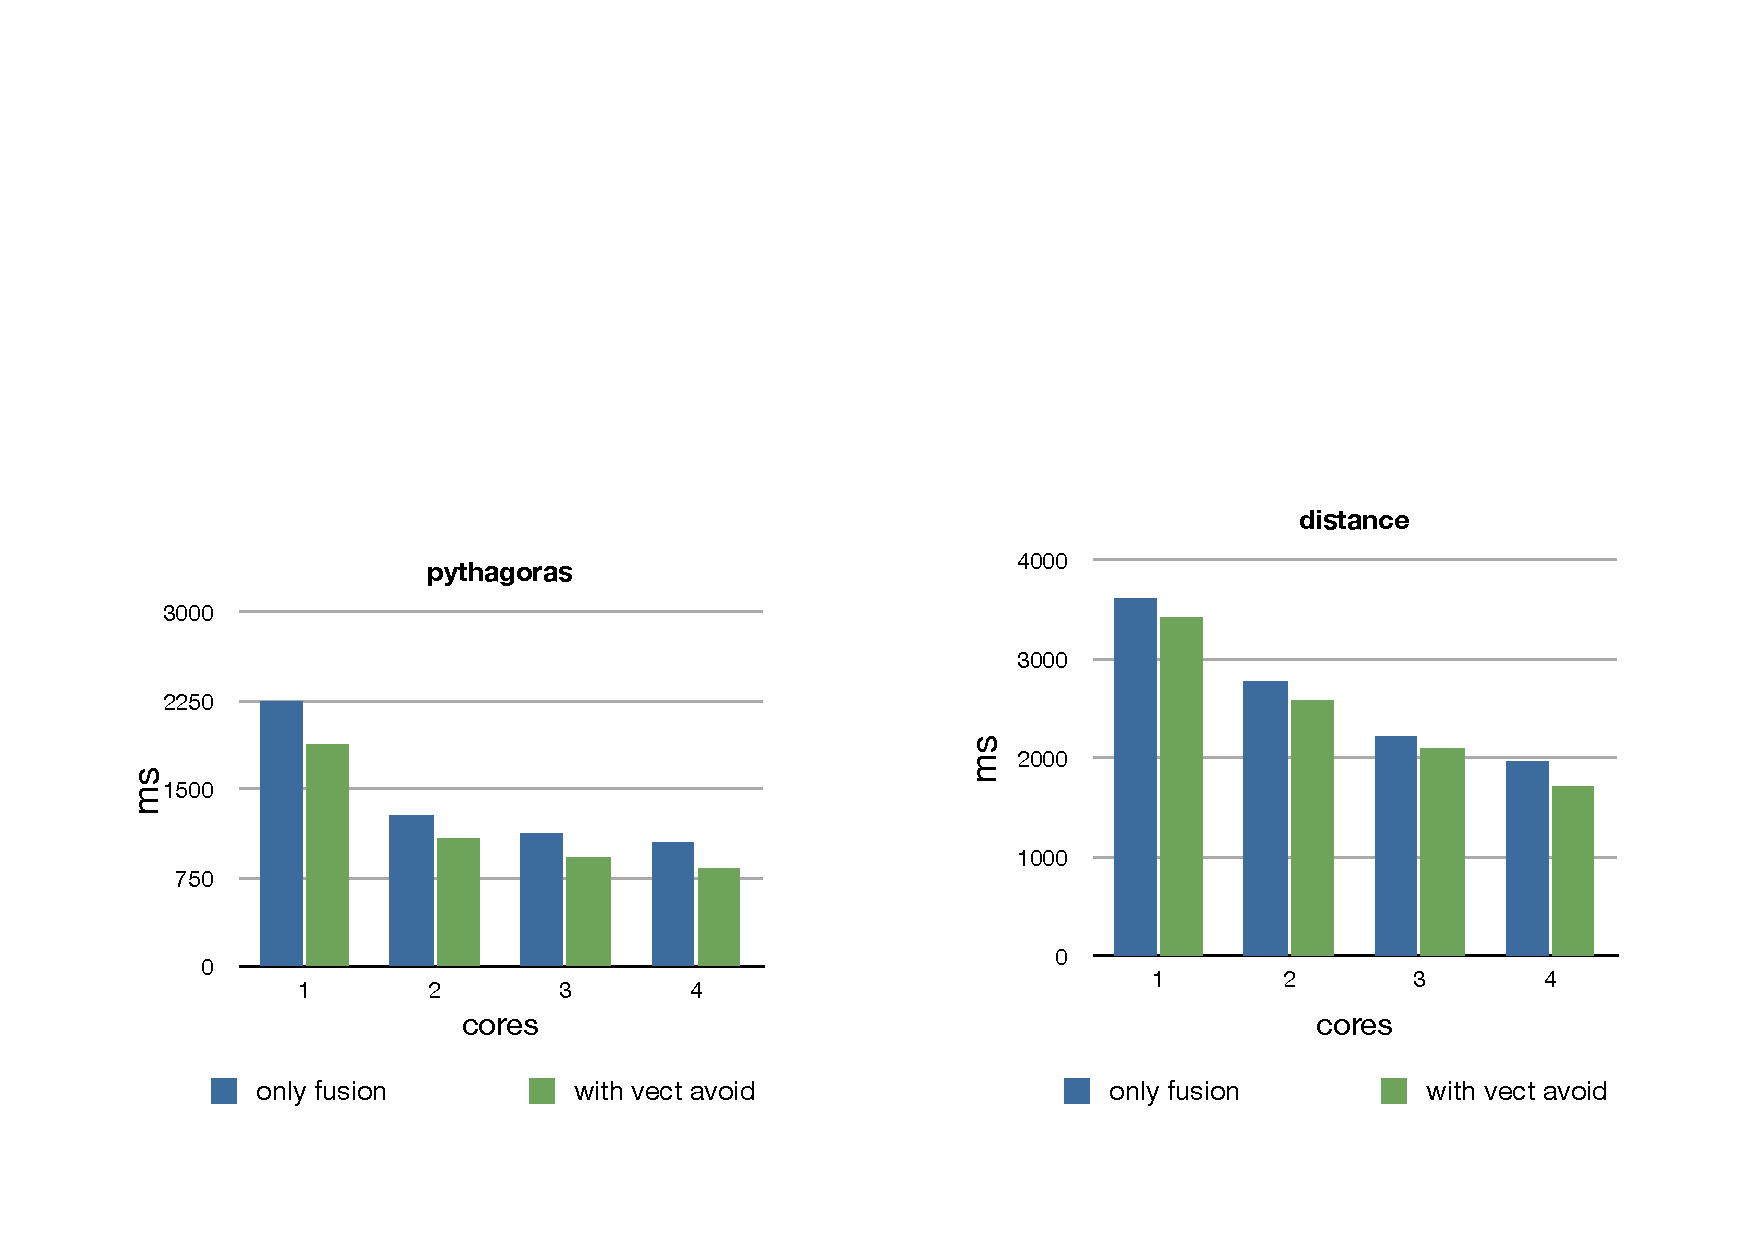
\includegraphics[scale=0.6, trim=0cm 2cm 0cm 8cm, clip]{data/DistancePythagoras.pdf}
\caption{Runtimes of the \texttt{pythagoras} and \texttt{distance} functions on vectors of $10^8$ floating-point numbers}
\label{Figure:distancePythagoras}
\end{figure*}
%
Our first two benchmark programs investigate the case where stream fusion~\cite{coutts:rewriting-strings, coutts:stream-fusion} is able to complete fuse a chain of array traversals. Specifically, we measure the running time of the following two functions when used in parallel --- that is, we measure @zipWith pythagoras xs ys@ and @zipWith distance xs ys@, where @xs@ and @ys@ are vectors containing $10^8$ @Double@ values:
%
\begin{quote}\small
\begin{alltt}
pythagoras x y
  = sqrt (x * x + y * y + 2 * x * y)

distance (xo, yo) ((x1, y1), (x2, y2))
  = (x1 - xo) * (y2 - yo) - (y1 - yo) * (x2 - xo)
\end{alltt}
\end{quote}
%
In our current implementation, the @Scalar@ class does not yet have an instance for pairs. Hence, vectorisation avoidance cannot use @zipWith_scalar@ on the entire body of @distance@. Instead it encapsulates the body of
the innermost case expression (performing pattern matching on the pairs); so, the code has the following structure after encapsulation:
%
\begin{quote}\small
\begin{alltt}
distance xy0 xy =
 case xy0 of (x0, y0) -> 
  case xy of (xy1, xy2) -> 
   case xy1 of (x1, y1) ->
    case xy2 of (x2, y2) -> 
     (\(\lambda\) x0 y0 x1 y1 x2 y2. 
       (x1 - x0) * (y2 - y0) - (y1 - y0) * (x2 - x0)) 
     x0 y0 x1 y1 x2 y2
\end{alltt}
\end{quote}
%
Given that the additional array traversals introduced by vectorisation of @pythagoras@ and @distance@ can be completely eliminated by array fusion, we might expect that vectorisation avoidance does not provide any additional benefit. However, the graph displayed in Figure~\ref{Figure:distancePythagoras} shows that vectorisation avoidance does improve performance slightly. This is as fusion results in slightly more complex loops than vectorisation avoidance.

According to the graph, the two benchmarks don't scale particularily well. In our opinion, this is as the code is memory bound --- i.e., the full floating-point performance of the processor is not exploited as the processor has to wait for the memory-subsystem to fetch the operands.

\subsection{Fusion and vectorisation avoidance together}

\begin{figure*}
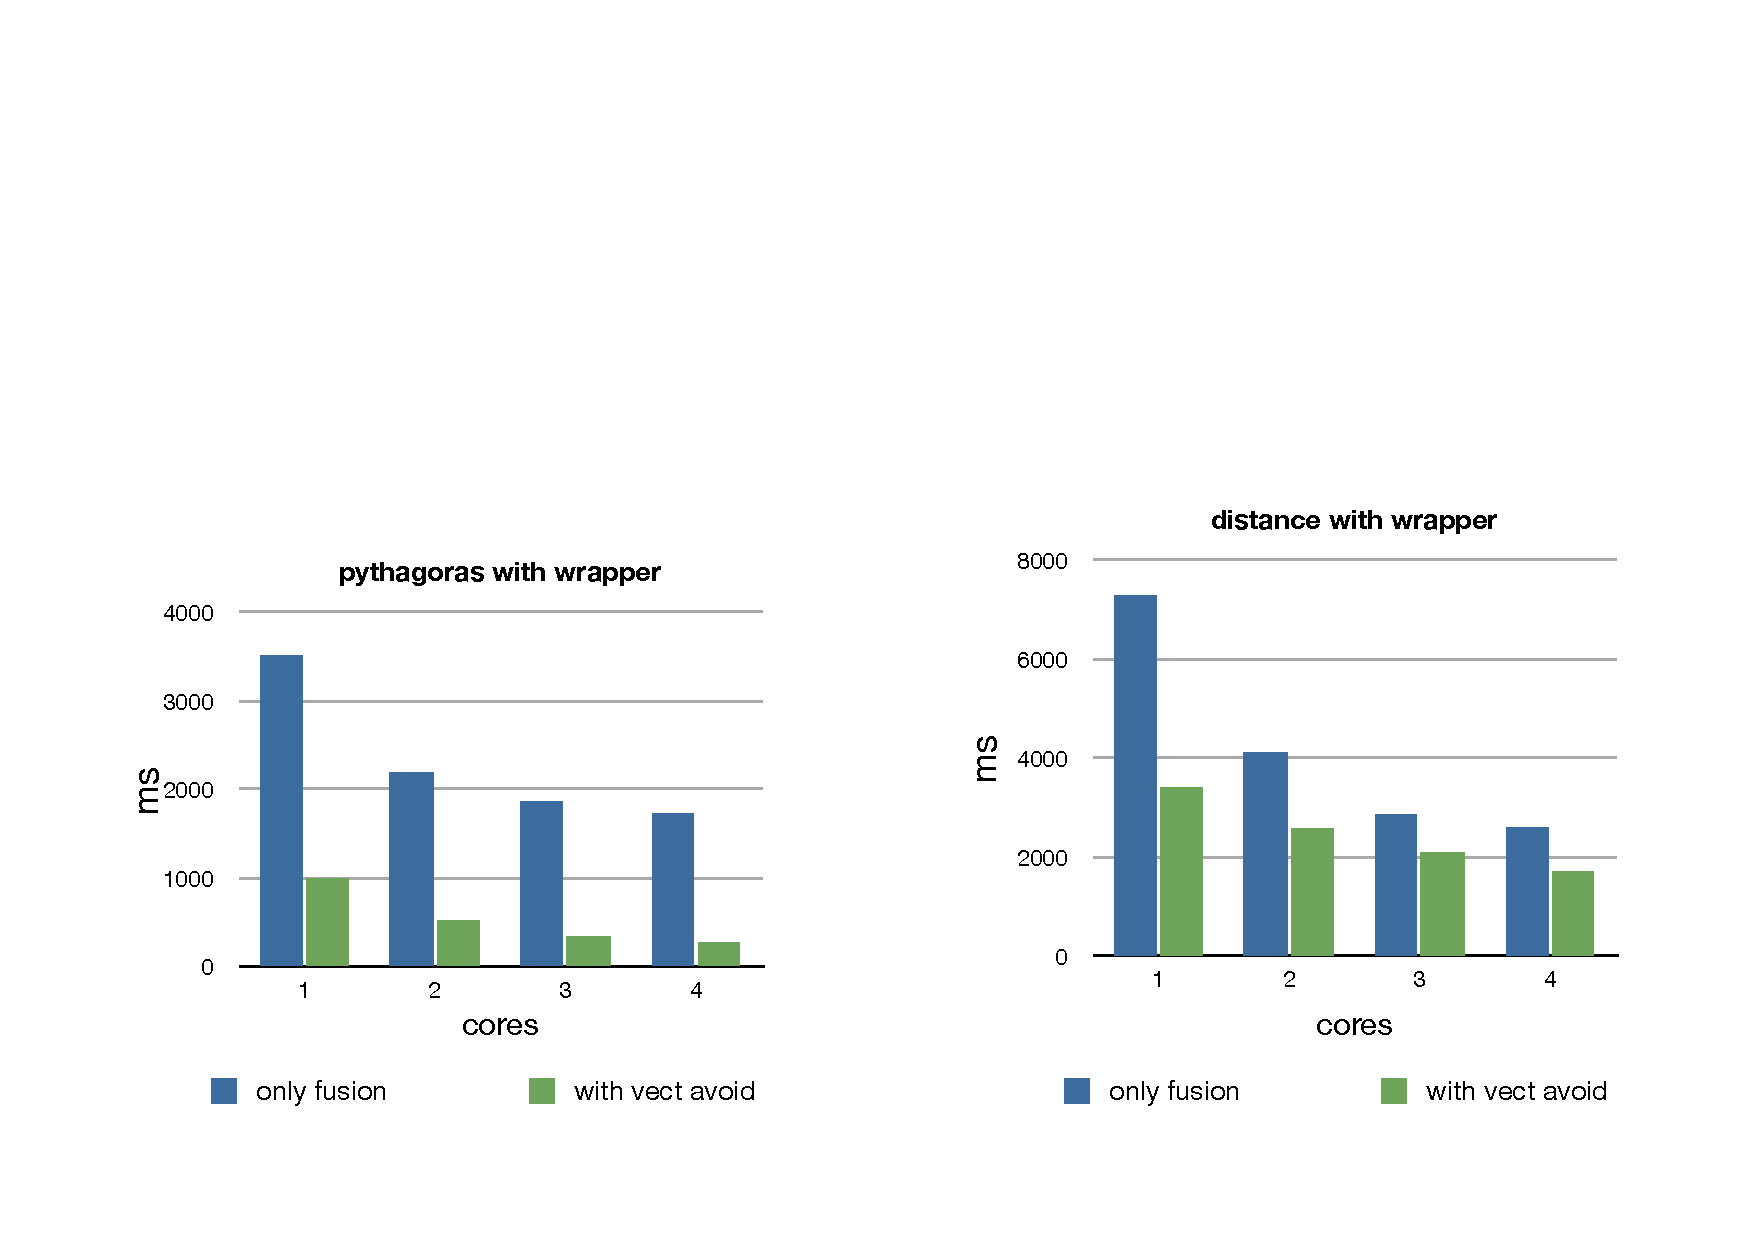
\includegraphics[scale=0.6, trim=0cm 2cm 0cm 8cm, clip]{data/DistPythagorasInl.pdf}
\caption{Runtimes of the \texttt{pythagoras} and \texttt{distance} functions \emph{with wrappers} on vectors of $10^8$ floating-point numbers}
\label{Figure:distancePythagorasInl}
\end{figure*}
%
In the previous benchmark, we measured the performance of @zipWithP pythagoras xs ys@ by itself (and the same with @distance@). Next, we have a look at that same code sandwiched between a producer (enumerating the arrays consumed by the @zipWithP@) and a consumer (summing up the result array with @sumP@); so, we have got
%
\begin{quote}\small
\begin{code}
sumP (zipWithP pythagoras 
               (enumFromToP 1 (10^8)) 
               (enumFromToP 1 (10^8)))
\end{code}
\end{quote}
%
Ideally, we would like the whole pipeline to fuse into a single loop that computes the final sum without creating any intermediate arrays. Looking at the graph in Figure~\ref{Figure:distancePythagorasInl} that does happen for the @pythagoras@ benchmark with vectorisation avoidance enabled. However, with fusion alone, performance is worse by more than a factor of 3. Array fusion by itself did not manage to eliminate the entire pipeline, whereas the combination of array fusion with vectorisation avoidance did that successfully leading to a dramatic performance improvement. Once the pipeline fuses completely, the code also scales better --- as there are no more intermediate structures, the memory-access bottleneck vanishes.

Why is fusion by itself not successful at removing all intermediate structures? In the lifted code, the arrays produced by the enumerations are shared, as the arguments to @pythagoras@ are used multiple times in the body. This hampers inlining, and hence, stream fusion. With vectorisation avoidance, all sharing is in the code that isn't vectorised, so this problem does not arise.

In the case of @distance@, vectorisation avoidance is also a clear improvement. However, it is less dramatic as the remaining pattern matching of the argument pairs (discussed in the previous subsection) prevents fusion of the entire pipeline.

\subsection{Conditionals}

\begin{figure*}
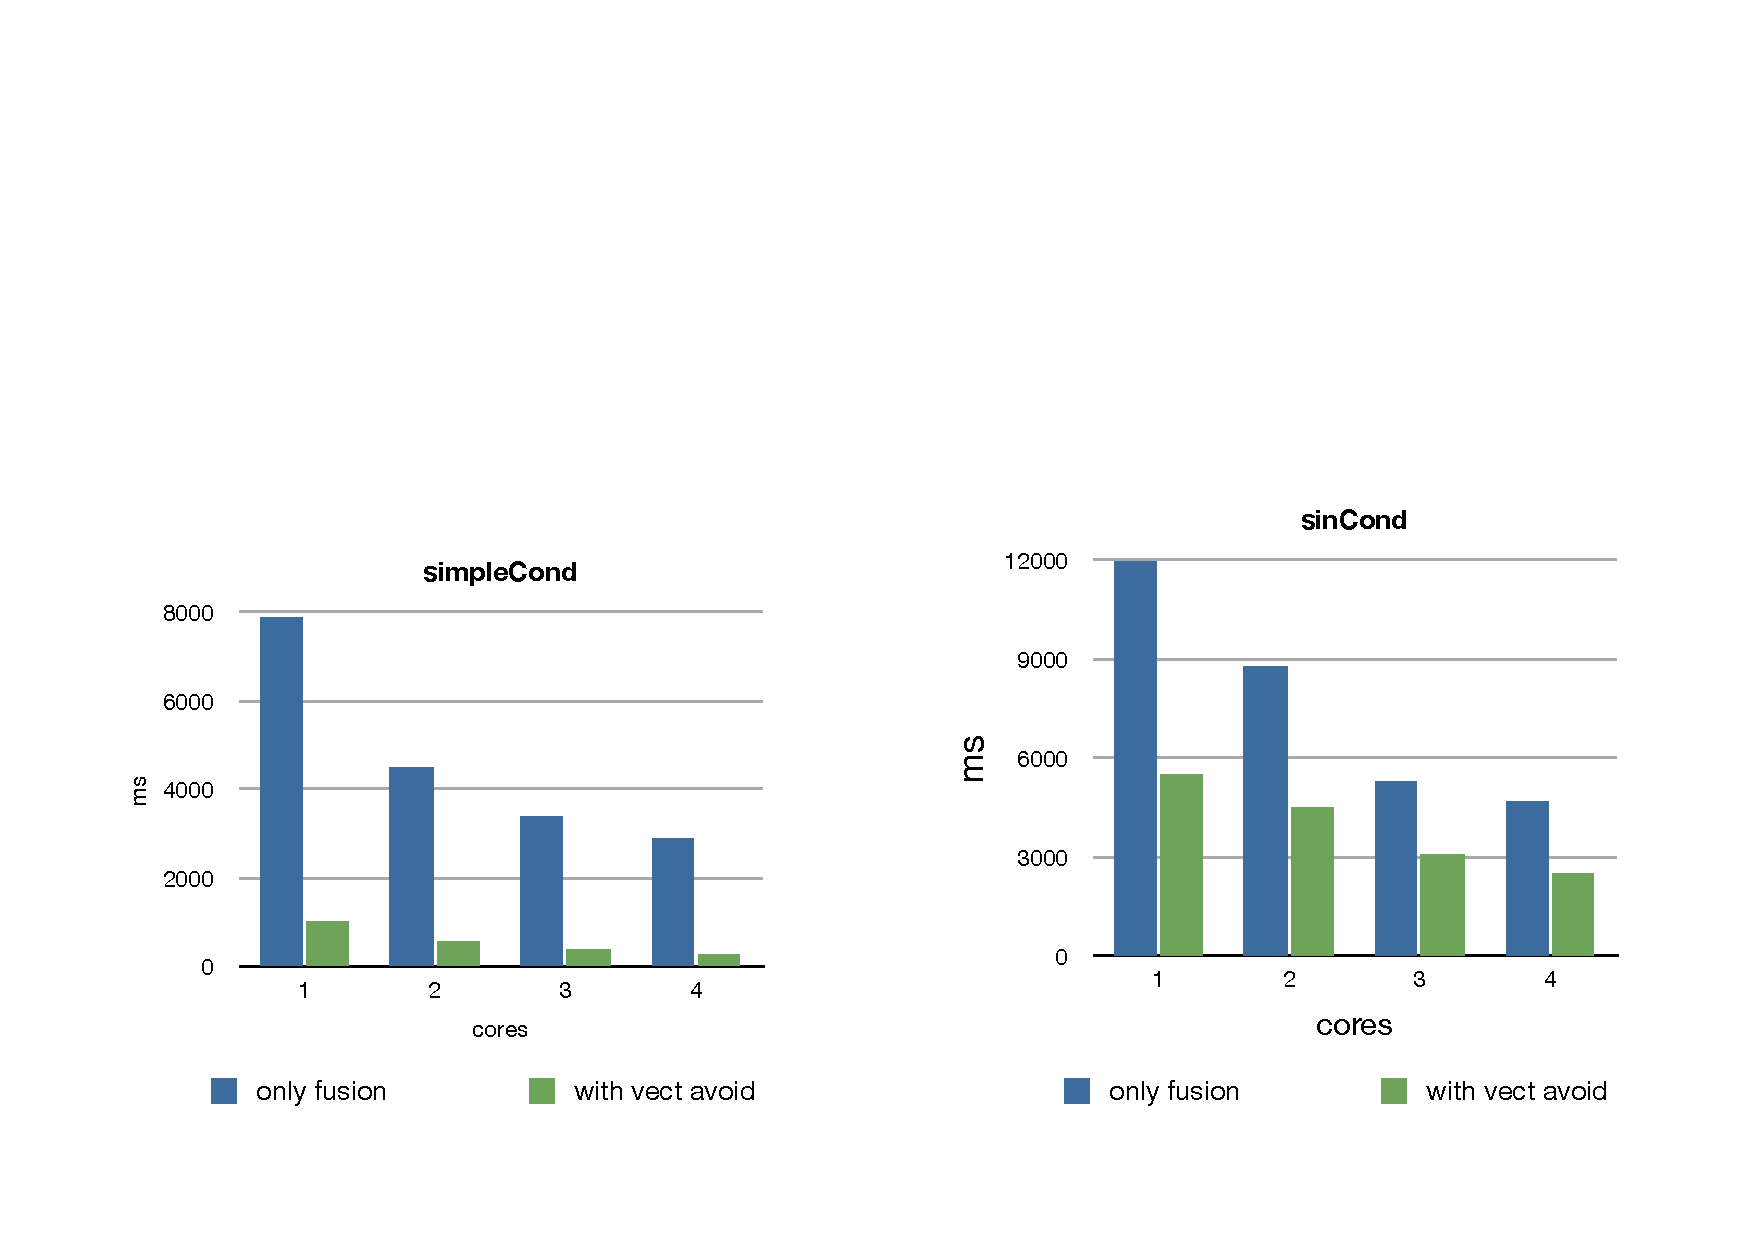
\includegraphics[scale=0.6, trim=0cm 2cm 0cm 8cm, clip]{data/Conditional.pdf}
\caption{Runtimes of the \texttt{simpleCond} and \texttt{sinCond} functions on vectors of $10^8$ \texttt{Int}s and \texttt{Double}s, respectively}
\label{Figure:Conditional}
\end{figure*}
%
Fully vectorising conditionals is expensive due to the @spliPA@ and @combinePA@ operations. On the other hand, vectorised conditionals balance load very well, whereas if vectorisation is avoided, we might suffer from load imbalance. To assess the impact of vectorisation avoidance on conditionals, we measured @mapP simpleCond xs@ and @mapP sinCond xs@, for arrays with $10^8$ elements, where
%
\begin{quote}\small
\begin{alltt}
simpleCond x = if (x `mod` 2 == 0) 
               then 3 * x 
               else 2 * x

sinCond n = if (x < n / 2) 
            then  x 
            else sin (sin (sin (2 * x)))
\end{alltt}
\end{quote}
%
We chose the input array to contain the increasing sequence of 1 to the size of the array. Hence, for @simpleCond@, we have no load imbalance with vectorisation avoidance, whereas @sinCond@ has a severe load imbalance as we execute the then-branch on the first half of elements and the else-branch on the other half.

As expected, the graph in Figure~\ref{Figure:Conditional} shows that vectorisation avoidance for conditionals is a big improvement when there is no load imbalance. However, even with a severe load imbalance, vectorisation avoidance is still an advantage for small numbers of cores. Nevertheless, with vectorisation avoidance, scalability suffers in case of load imbalance; hence, it would be worthwhile to enable the programmer to determine the behaviour of the vectoriser with a pragma.

% In the second example, the time necessary for evaluating the two branches differs, and applied to the ordered array we use as input, there is a significant load imbalance, as the alternative is only called on elements of the second half of the array. In practice, we find that this degree of imbalance is fairly rare. As we would expect, the relative speedup for the fully vectorised version is slightly better (2.7) than for the one compiled with vectorisation avoidance (2.2), but in absolute terms, the latter version is, even on four PEs. more the 50\% faster. It may seem surprising that the difference is not bigger. However, redistributing the data involves communication, which in turn is more expensive the more
% PEs are involved, putting a cap on the possible speedup.
% In general, vectorisation avoidance will yield the better results for scalar conditionals with constant work complexity. However, it does not seem reasonable to
% stick with one fixed compilation strategy for the whole program in this case, as it is definitely possible to write programs for which either would be a bad choice. The programmer should have the possibility two enforce a particular strategy via a code pragma. We have not implemented such a pragma yet, but the transformation could be adapted easily to handle this.

\subsection{Recursive Functions}

\begin{figure}
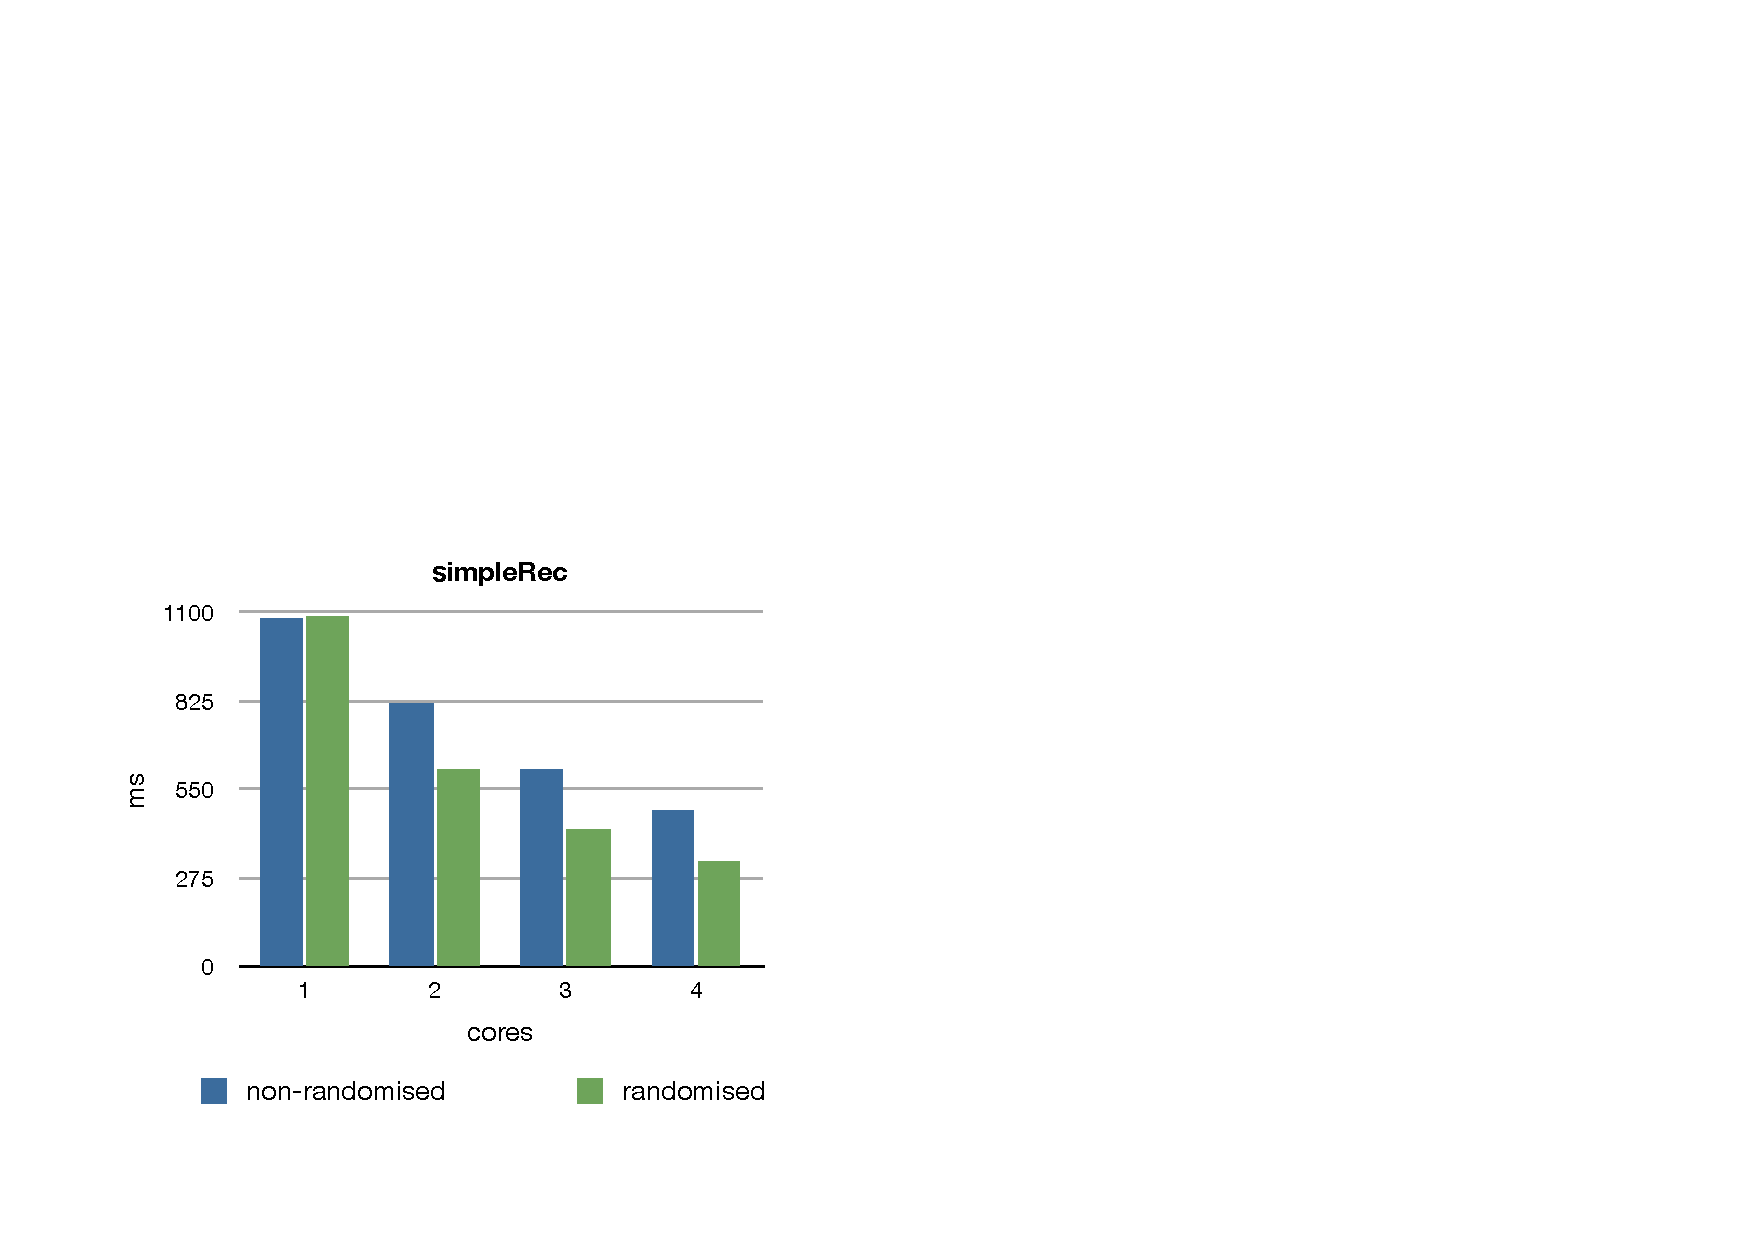
\includegraphics[scale=0.6, trim=0cm 2cm 0cm 9cm, clip]{data/Recursion.pdf}
\caption{Runtimes of \texttt{simpleRec} on vectors of $10^5$ \texttt{Double}s with and without randomisation}
\label{Figure:Recursion}
\end{figure}
%
The question of load imbalance becomes even more pressing when the work complexity of a function depends on the array element it is applied to, as in
%
\begin{quote}\small
\begin{alltt}
simpleRec x = if (x < 5) 
              then x 
              else simpleRec (x - 5)
\end{alltt}
\end{quote}
%
Interestingly, in the case of a tail recursive function, the benefit of vectorisation avoidance is even greater, as vectorisation prevents the code generator compiling the recursion into a simple loop. For the admittedly extreme case of @simpleRec@, where there is no work in the recursive steps, the fully vectorised version is two orders of magnitude slower than when we use vectorisation avoidance.

Unfortunately, when mapping @simpleRec@ over an array containing the increasing sequence of 1 to the size of the array, load imbalance is also significant. Vectorisation of @simpleRec@ provides load balancing, but, in this example, with a prohibitively expensive constant factor. An alternative to full vectorisation in such cases is to apply vectorisation avoidance, but to randomise the input vector. The graph in Figure~\ref{Figure:Recursion} suggests that this is a worthwhile strategy. Currently, a programmer needs to do it explicitly, but we plan to investigate automatic randomisation.

\subsection{Calculating accelerations}

\begin{figure}
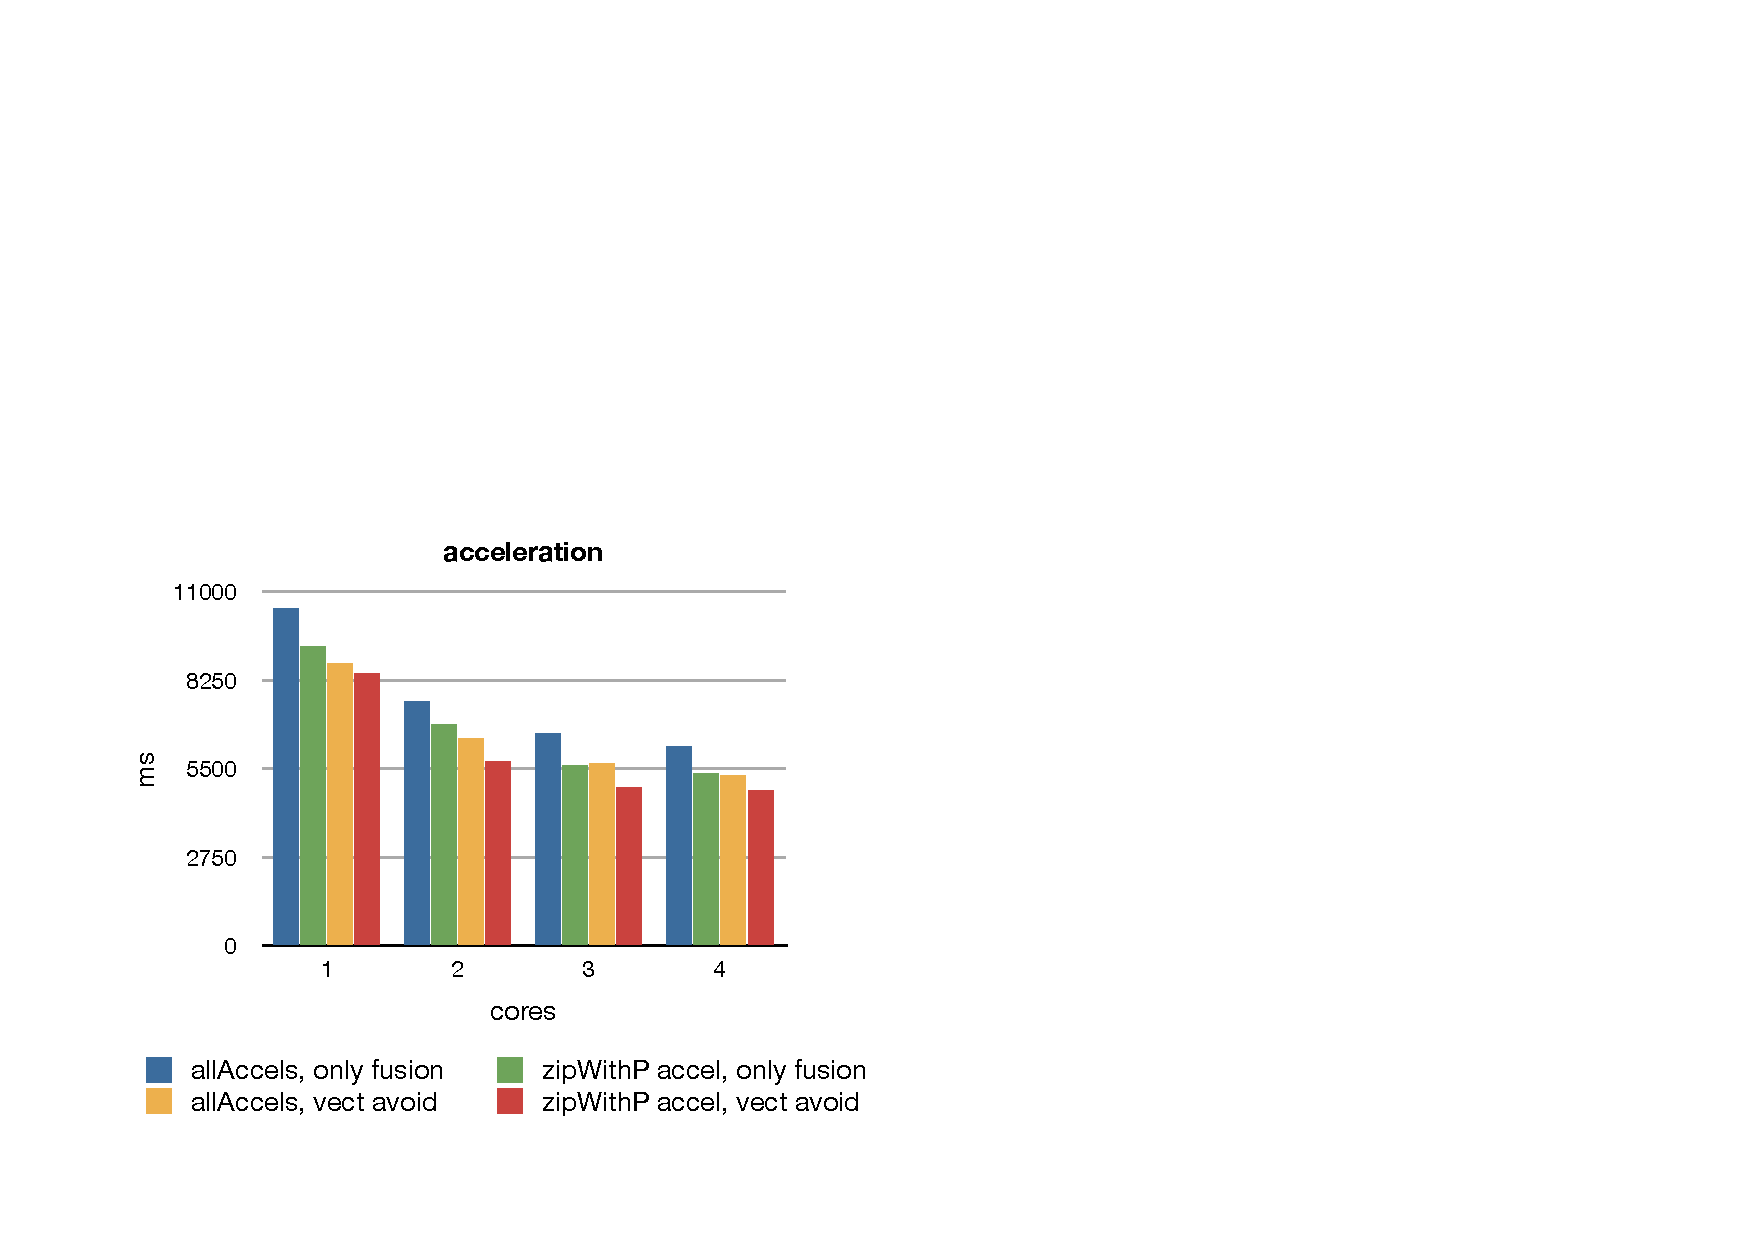
\includegraphics[scale=0.6, trim=1.5cm 2cm 0cm 9cm, clip]{data/Accel.pdf}
\caption{Runtimes of \texttt{allAccels} and \texttt{zipWithP accels} computing $10^8$ interactions}
\label{Figure:Accel}
\end{figure}
%
Figure~\ref{Figure:Accel} displays the running times for computing the acceleration of $10^8$ mass point interactions with and without vectorisation avoidance. It does so in two ways. Firstly, by using @allAccels@ on $10^4$ mass points (it implements a quadratic algorithm); and secondly, by directly using @zipWithP accel@ on two arrays of $10^8$ mass points. The main difference between these two computations is that @allAccels@ also computes $2*10^4$ parallel sums. Hence, it is not surprising that @allAccels@ is slower than @zipWithP accel@ across the board.

However, it is interesting to see that the gain due to vectorisation avoidance is higher in the case of @allAccels@, where it is 11\% on a single core, than for @zipWithP accel@, where it is 3\%. The reason is as for @pythagoras@ and @distance@ with wrappers. Fusion of the acceleration computation with @sumP@ is more effective with vectorisation avoidance.

Note also that, as previously mentioned, the @Scalar@ class in our current implementation does not yet include pairs. Hence, the vectorisation of @accel@ cannot yet be entirely avoided (c.f., the explanation for @distance@ in Section~\ref{sec:simple-arith}). We expect the gain to be even more pronnounced once that is the case.

\subsection{Compilation time}

We argued that, apart from producing faster code, vectorisation avoidance also produces simpler code which requires fewer subsequent optimisations.  This, in turn, should result in shorted compilation times.  For the examples presented in this section, overall compilation was about 25\% faster when vectorisation avoidance was enabled.

\section{Related Work}
\label{sec:related}

We are not aware of any other work that attempts to selectively avoid vectorisation in higher-order programs. However, in a recent port of Blelloch's original NESL system to GPUs~\cite{bergstrom-reppy:ndp-gpu}, the code for NESL's virtual vector machine, called VCODE, is analysed to fuse sequences of lifted arithmetic operations. This is selectively \emph{undoing} some vectorisation, albeit in a first-order setting. Much like our old stream fusion system, it cannot undo the vectorisation of conditionals or recursive functions.

Manticore is an implementation of nested data parallelism that foregoes vectorisation entirely and instead relies on dynamic methods, such as work stealing and lazy tree splitting~\cite{bergstrom-etal:lts}. Similarly, Blelloch et al.~\cite{BGM99,Spoonhower:2010} investigated alternatives to flattening based on multi-threading. Based on the scheduling strategy, they were able to establish asymptotic bounds on time and space for various forms of parallelism, including nested data parallelism. 

Overall, there are two general approaches to implementing nested data parallelism. Approaches based on multi-threading naturally fit the execution model of MIMD machines, such as multicore processors. However, they need to make an effort to ensure load balancing (e.g., by using work stealing) and to agglomerate operations on successive array elements (to get efficient loops). The alternative is vectorisation, which in its pure form produces pure SIMD programs. Hence, they need to make an effort to increase locality (e.g., by array fusion). It appears as if we need a hybrid approach, and the question is whether to start from the MIMD or SIMD end. We chose to start from SIMD and relax that using vectorisation avoidance, as disucssed here, and also a more flexible array representation as discussed in a companion paper~\cite{lippmeier:work-efficient}.
% -----------------------------------------------------------------------------
\paragraph{Acknowledgements.}
This work was supported in part by the Australian Research Council under grant number LP0989507. 

\bibliographystyle{abbrvnat}
\bibliography{Main}

\end{document} 

